% ==================================================================
% Master file
% ==================================================================

\documentclass[12pt,a4paper,oneside]{scrreprt}

% ---------- Language & Encoding ----------
% (für LuaLaTeX: keine inputenc/fontenc)
\usepackage{fontspec}
\defaultfontfeatures{Ligatures=TeX}
\setmainfont{Latin Modern Roman}
\setsansfont{Latin Modern Sans}
\setmonofont{Latin Modern Mono}
\usepackage[english]{babel}
\usepackage{csquotes}

% --- Unicode -> LaTeX Mappings (fix build) ---
\usepackage{newunicodechar}
\newunicodechar{′}{\ensuremath{^{\prime}}}   % U+2032 prime
\newunicodechar{⇒}{\ensuremath{\Rightarrow}} % U+21D2
\newunicodechar{→}{\ensuremath{\to}}         % (falls benutzt)
\newunicodechar{≤}{\ensuremath{\le}}         % (falls benutzt)
\newunicodechar{≥}{\ensuremath{\ge}}         % (falls benutzt)
\newunicodechar{±}{\ensuremath{\pm}}         % (falls benutzt)

% Build-Metadaten (aus CI befüllt; lokal Fallback)
\IfFileExists{buildmeta.tex}{\input{buildmeta.tex}}{%
  \def\BuildRun{DEV}\def\BuildSHA{local}\def\BuildDate{\today}%
}

% ---------- Layout & Aesthetics ----------
\usepackage{geometry}
\geometry{left=3cm,right=2.5cm,top=2.5cm,bottom=3cm}
\usepackage{setspace}\onehalfspacing
\usepackage{microtype}

% ---------- Math, Tables, Units ----------
\usepackage{amsmath,amssymb,mathtools}
\usepackage{siunitx}\sisetup{detect-all=true}
\usepackage{booktabs,array,multirow}

% ---------- Graphics ----------
\usepackage{graphicx,subcaption,caption}
\captionsetup{labelfont=bf}
\graphicspath{{figures/}{figures/fig/}}
% \setkeys{Gin}{draft=true} % falls Bilder fehlen

% ---------- Links & Clever refs ----------
% Links & Clever refs
\usepackage{xcolor}
\definecolor{linkblue}{HTML}{0A66C2}
\usepackage{hyperref}
\hypersetup{colorlinks=true,linkcolor=black,citecolor=linkblue,urlcolor=linkblue}
\usepackage[nameinlink,noabbrev]{cleveref}

% Math in moving arguments (section titles, captions) -> ASCII fallback
\pdfstringdefDisableCommands{%
  \def\Cout{Cout}%
  \def\sinIn{sinIn}%
  \def\kO{kappaO}%
  \def\Theta{Theta}%
  \def\Rightarrow{=>}%
  \def\;{}%
  \def\({}%
  \def\){}%
}
% ---------- Plots (optional) ----------
\usepackage{pgfplots}
\pgfplotsset{compat=1.18}

% ---------- Bibliography ----------
\usepackage[backend=biber,style=authoryear,maxbibnames=99,giveninits=true]{biblatex}
\addbibresource{references.bib}

% ---------- TODOs (toggle) ----------
\newif\ifdraft \draftfalse
\ifdraft\usepackage{todonotes}\setlength{\marginparwidth}{2cm}\else\usepackage[disable]{todonotes}\fi

% ---------- Helper Macros ----------
\usepackage{xparse}
% failsafe \addfig: bricht nicht ab, wenn Bild fehlt
\NewDocumentCommand{\addfig}{O{htbp} m m m O{0.9}}{%
  \begin{figure}[#1]\centering
    \IfFileExists{#2}{\includegraphics[width=#5\linewidth]{#2}}%
    {\fbox{\parbox{.9\linewidth}{\centering Missing file: #2}}}%
    \caption{#3}\label{#4}
  \end{figure}}

% concept boxes
\newenvironment{insight}{\par\vspace{0.5em}\noindent\textbf{Insight.}\ }{\par\vspace{0.5em}}
\newenvironment{implication}{\par\vspace{0.5em}\noindent\textbf{Implication.}\ }{\par\vspace{0.5em}}
\newenvironment{limitation}{\par\vspace{0.5em}\noindent\textbf{Assumptions \\ \& Limitations.}\ }{\par\vspace{0.5em}}

% notation
\newcommand{\sinIn}{s_{\mathrm{in}}}
\newcommand{\Cout}{C_{\mathrm{out}}}
\newcommand{\kO}{\kappa_{\mathrm{O}}}

% Backward-compat für alte Font-Befehle (KOMA-safe)
\DeclareOldFontCommand{\rm}{\normalfont\rmfamily}{\mathrm}
\DeclareOldFontCommand{\sf}{\normalfont\sffamily}{\mathsf}
\DeclareOldFontCommand{\tt}{\normalfont\ttfamily}{\mathtt}
\DeclareOldFontCommand{\bf}{\normalfont\bfseries}{\mathbf}
\DeclareOldFontCommand{\it}{\normalfont\itshape}{\mathit}
\DeclareOldFontCommand{\sc}{\normalfont\scshape}{\relax}

% ==================================================================

\begin{document}
\begin{titlepage}
  \centering
  {\Large Master Thesis (Hypothesis-Driven, Physically Anchored)}\\[0.6em]
  {\huge\bfseries Roles, Thresholds, and Counting Time}\\[0.25em]
  {\Large\bfseries From Ur-Fabric to Cosmos, Life, Mind \& AI}\\[1.0em]
  {\large A Dimension-Agnostic, Falsifiable Role Calculus}\\[-0.2em]
  {\small (\,O: orientation/transport,\ G: binding/structuring,\ K:=O$\!\circ$G;\ $t:=C[\tau^K]$\,)}\\[2.0em]

  \begin{tabular}{@{}ll@{}}
    Author: & Tim Brötzmann \\
    Submission date: & \today \\
    Build: & Run \BuildRun\ (\BuildSHA) — \BuildDate \\
  \end{tabular}

  \vfill
  \IfFileExists{figures/logo-placeholder}{\includegraphics[width=0.28\linewidth]{figures/logo-placeholder}}{}
\end{titlepage}

\pagenumbering{roman}

\chapter*{Abstract}
We propose a dimension-agnostic \emph{role calculus} with two primitives—%
\emph{orientation/transport} $O$ and \emph{binding/structuring} $G$—and a non-acting reader $C$.
The reader makes roles visible and \emph{counts}: $\tau^O$ counts $O$-events, $\tau^K$ counts overlap-events $K:=O\!\circ G$, and macroscopic time is the coarse continuation $t:=C[\tau^K]$.
No new forces are introduced; sector avatars (gravity, electrostatics, radiation, networks) appear as weak-field limits of the same roles.

Two thresholds organize dynamics: a \emph{seed} threshold $\Theta$ (nucleation) and a \emph{persistence} threshold $\sigma_c$ (long-lived channels). This yields three parameter-light, falsifiable signatures:
\emph{T1} (orientation avatar): inner/outer slopes $(+1,-2)$ with a parameter-free inside–outside identity $C_{\mathrm{out}}/s_{\mathrm{in}}=a^3$ (generalized to $D$ spatial dimensions as $(+1,-(D\!-\!1))$ and $a^{D}$);
\emph{T2} (bridge): a finite cross-coherence band $0<C_1(k)<1$ between flows and potentials, removed by phase-shuffle nulls;
\emph{T3} (thresholds): nucleation/persistence hysteresis with loop area $\mathcal A_{\rm loop}>0$.

We map the same roles across layers—Ur-fabric $\rightarrow$ cosmos $\rightarrow$ molecules $\rightarrow$ life $\rightarrow$ mind/AI.
Near black holes, a “release shell’’ ($r\!\sim\!1.2$–$10\,r_s$) acts as a concentration tree (trunk/channels/knots/seeds); we specify \emph{B-tests} (ringdown echoes, extra $C_1(k)$ peak near the photon ring, HFQPO over-ISCO) to detect $K$-events.
For life, we formalize the \emph{Keim window} $\Delta\mu_{\rm eff}\!\gtrsim\!\Theta_{\rm eff}=\Theta/[k(|w_1|\!+\!|w_2|)]$, a \emph{viability bound}
$\varepsilon_{\rm req}=E_{\rm req}/(N_{\rm orb}p_{\rm survive})$,
the \emph{error threshold} $Q^L s>1$, and a compartment retention trade-off.
Existential stability is summarized by
$\mathrm{SEC}\propto (\tau^K/(S{+}N))\,(T_{\rm above}/W)$.
Phase/superposition is treated operationally: geometry can compress phase (coherence $\uparrow$) to cross thresholds ($\Delta\tau^K=1$), otherwise no new counts accrue.

The framework is deliberately minimal and falsifiable: it constrains microphysics via cross-scale role regularities and yields tests that hold in strict $3{+}1$D while remaining compatible with higher-$D$ hypotheses (which would only renormalize exponents/couplings rather than introduce new primitives).

\chapter*{Keywords}
role calculus; orientation $O$; binding $G$; composition $K{:=}O\!\circ G$; counting time $t{:=}C[\tau^K]$; $\tau^O$; $\tau^K$; thresholds $\Theta,\sigma_c$; hysteresis; SEC (existential stability); cross-coherence $C_1(k)$; decoupling band; parameter-free identity $C_{\mathrm{out}}/s_{\mathrm{in}}=a^{3}$ (and $a^{D}$); dimensional diagnostic; stacking; gravity/electrostatics avatars; baryon conditioning; black-hole release shell; EHT polarization/closure phase; HFQPO over-ISCO; ringdown echoes; Keim window $\Delta\mu_{\rm eff}\!\gtrsim\!\Theta_{\rm eff}$; viability bound $\varepsilon_{\rm req}$; error threshold $Q^L s>1$; compartment retention; coordination plateaus (C$_2$); apex keim (Human→AI); guardrails; universality-class stance; falsifiability; dimension-agnostic.

\tableofcontents
\listoffigures
\listoftables
\clearpage
\pagenumbering{arabic}

\part{Introduction}

\section*{Plain-language overview}
This work asks a simple question with big consequences: \emph{Are two roles enough to organize what we see across physics and biology?} 
We call them \textbf{orientation/transport} ($O$) and \textbf{binding/structuring} ($G$). 
They are not new forces; they are \emph{what processes do}. 
A reader $C$ makes these roles visible and \emph{counts}: $\tau^O$ counts $O$-events; $\tau^K$ counts overlap-events $K:=O\!\circ G$; macroscopic time is the coarse continuation $t:=C[\tau^K]$. 
From that vantage point, familiar inverse-square laws, potential wells, flows, membranes, neurons, markets—look like \emph{the same grammar} at different scales.

What is genuinely new here is not a metaphysical claim but a \emph{testable} one: in weak fields, stacks around approximately spherical deficits must show a paired slope signature $(+1,-2)$ and a parameter-free inside–outside identity. 
Flows and potentials should partially line up (a finite $0<C_1(k)<1$ band), and thresholded systems should exhibit nucleation–persistence hysteresis. 
Those three signatures (T1–T3) are our through-line from Ur-fabric to cosmos, life, mind, and AI.

\subsection*{What is new here (in one page)}
\begin{enumerate}
  \item \textbf{Counting time.} We operationalize time as counting of real events: $\tau^O$, $\tau^K$, $t=C[\tau^K]$. $C$ \emph{does not act}; it reads.
  \item \textbf{Dimension-agnostic weak-field law.} The orientation avatar yields inner/outer slopes and a parameter-free identity. In 3D this is $(+1,-2)$ with $C_{\mathrm{out}}/s_{\mathrm{in}}=a^3$; in $D$ dimensions it generalizes to $(+1,-(D\!-\!1))$ and $a^{D}$.
  \item \textbf{Cross-coherence bridge.} Flows vs.\ potentials exhibit a finite coherence band $0<C_1(k)<1$—\emph{not} a perfect lock—organizing residuals and scale-coupling.
  \item \textbf{Thresholds and hysteresis.} Two thresholds matter: a seed threshold $\Theta$ (nucleation) and a persistence threshold $\sigma_c$ (long-lived channels). Their operational face is a hysteresis loop with area $\mathcal A_{\rm loop}>0$.
  \item \textbf{Same roles across layers.} Ur-fabric $\to$ cosmos (e.g.\ near-horizon “release shells”), $\to$ molecules \& life (Keim window, compartments), $\to$ mind/AI (coordination plateaus, apex keim). No new primitives are added; only avatars and parameters change.
\end{enumerate}

\subsection*{Key questions}
\begin{enumerate}
  \item \emph{Minimality.} Are $O$ and $G$ sufficient as role primitives once time is treated as counting via $C$?
  \item \emph{Falsifiability.} Do data exhibit T1 (paired slopes $+1/-2$ and identity), T2 (finite $C_1(k)$ band with null removal), and T3 (hysteresis with $\mathcal A_{\rm loop}>0$)?
  \item \emph{Bridging.} Can the same tests diagnose overlap events from Ur-fabric to black-hole environs, to prebiotic chemistry, to neural coordination?
  \item \emph{Robustness.} Do results hold in strict $3{+}1$D—and how would higher-$D$ hypotheses show up (exponent/coupling shifts) without adding new primitives?
\end{enumerate}

\begin{insight}
\textbf{Role vs.\ mechanism.} We separate \emph{what} a process does ($O,G$) from \emph{how} it is implemented (microphysics). This keeps the language compact across domains and puts tests first.
\end{insight}

\begin{implication}
\textbf{One toolkit, many layers.} If the role signatures persist, we gain a common diagnostic and reporting standard from gravity avatars to protocells to coordinated neural plateaus.
\end{implication}

\begin{limitation}
\textbf{Not a replacement for microphysics.} The role calculus constrains sector models via cross-scale regularities; it must \emph{earn} value by identities that survive measurement and null tests.
\end{limitation}

\subsection*{What we will test (map for the reader)}
\textbf{T1 Orientation (weak-field)}: $(+1,-2)$ slopes and $C_{\mathrm{out}}/s_{\mathrm{in}}=a^3$ (with $a^{D}$ generalization).\\
\textbf{T2 Bridge (cross-coherence)}: finite $0<C_1(k)<1$ band, removed by phase-shuffle nulls.\\
\textbf{T3 Thresholds (hysteresis)}: distinct on/off thresholds $(\Theta_\uparrow,\Theta_\downarrow)$ with loop area $\mathcal A_{\rm loop}>0$.\\[0.3em]
\emph{Context-specific hooks (later sections).} 
BH “tree’’ (B-tests: echoes, extra $C_1(k)$ near the photon ring, HFQPO over-ISCO); 
life “Keim window’’ ($\Delta\mu_{\rm eff}\gtrsim \Theta_{\rm eff}$), viability bound $\varepsilon_{\rm req}$, error threshold $Q^L s>1$, compartment retention; 
coordination plateaus (C$_2$) for mind/AI and apex keim with guardrails.

\part{Ur-Fabric: Core Calculus and Predictions}\label{part:ur}

\chapter{Triad, Primitive Roles, and Counting Time}\label{ch:ur-triad}

\section{Purpose and stance}\label{sec:ur-purpose}
\begin{insight}
\textbf{What we build.} A compact \emph{role calculus} with two primitives—%
\emph{orientation/transport} $O$ and \emph{binding/structuring} $G$—and a non-acting reader $C$. 
$C$ only \emph{makes roles visible and counts}: $\tau^O$ counts $O$-events; $\tau^K$ counts overlap-events $K:=O\!\circ G$; macroscopic time is the coarse continuation $t:=C[\tau^K]$.
\end{insight}

\begin{implication}
\textbf{Why roles (not new forces).} If many domains (gravity, electrostatics, radiation, networks, biology) share the same few \emph{role signatures}, we can test one grammar across scales with parameter-light criteria.
\end{implication}

\begin{limitation}
\textbf{Scope.} The calculus \emph{does not} replace microphysics; it constrains them via cross-scale regularities that must survive measurement and null tests.
\end{limitation}

\section{Assumptions and notation}\label{sec:ur-assumptions}
\textbf{Weak-field assumptions.} (A1) locality; (A2) isotropy; (A3) linear superposition.  
\textbf{Basis.} Substrate/contrast $(S,N)$.  
\textbf{Diagnostics.} $C_0$ (systemic coherence; non-operative), $C_1(k)$ (cross-coherence of bridge variables), $C_2$ (life-level coordination).  
A convenient intensity is
\begin{equation}
\sigma(O,G)=\alpha\|O\|^2-\beta\|G\|^2,\quad \alpha,\beta>0.
\end{equation}

\paragraph{Moderate universality (Assumption U).}
$O,G$ are primitive on the Ur-fabric. Higher layers (cosmos, life, human/AI) use \emph{avatars} $O_{\rm eff},G_{\rm eff}$ that preserve the algebraic roles and Gauss-type counting; curl/nonlinear corrections vanish in the weak-field limit.

\section{Phase, superposition, and reading}\label{sec:ur-phase}
Before $C$ reads, role-states can be coherently superposed over $(S,N)$:
\[
\lvert\psi\rangle=\cos\frac{\theta}{2}\lvert N\rangle+e^{i\phi}\sin\frac{\theta}{2}\lvert S\rangle.
\]
$\phi$ controls interference. $C$ projects to real counts (0/1) and accrues $\tau^O,\tau^K$. Geometry can \emph{compress phase} (good guidance/support), lengthening coherence and enabling a threshold-crossing event $\Delta\tau^K=1$; otherwise phase decoheres and no new counts accrue.

\section{Primitive process forms}\label{sec:ur-primitives}
Compositionally (diagnostic view),
\begin{equation}
O:=C_0\!\circ N\quad\text{(orientation/transport)},\qquad
G:=C_0\!\circ S\quad\text{(binding/structuring)},\qquad
K:=O\!\circ G\ \text{(overlap; non-commutative)}.
\end{equation}
Counting clocks: $\tau^O=\operatorname{ord}\{O_k\}$, $\tau^K=\operatorname{ord}\{K_k\}$, $t=C[\tau^K]$.

\section{Minimal orientation avatar (weak-field, \(D\) spatial dimensions)}\label{sec:ur-orientation}
Let $\mathbf v_O=\kappa_O\nabla\Omega$ be irrotational with Gauss counting on a deficit density $\rho_N$:
\begin{align}
\mathbf v_O&=\kappa_O\nabla\Omega, &&\text{(O1)}\\
\nabla\!\cdot\mathbf v_O&=S_D\,\kappa_O\,\rho_N 
\ \Longleftrightarrow\ \ \nabla^2\Omega=S_D\,\kappa_O\,\rho_N, &&\text{(O2)}
\end{align}
where $S_D$ is the $D$-sphere surface factor ($S_3=4\pi$). For a point source $n$:
\begin{equation}
\Omega(r)=-\frac{\kappa_On}{r^{D-2}},\qquad 
\mathbf v_O(r)=\frac{\kappa_On}{r^{D-1}}\,\mathbf e_r.\quad\text{(O3)}
\end{equation}
In $D\!=\!3$ this is the familiar inverse-square avatar.

\section{Geometric signatures around spherical deficits}\label{sec:ur-signatures}
For a homogeneous core radius $a$:
\begin{align}
\beta_O(r)&:=\frac{d\ln v_r}{d\ln r}=\begin{cases}+1,& r\le a,\\ -(D-1),& r\ge a,\end{cases}\label{eq:slopesD}\\
\frac{C_{\rm out}}{s_{\rm in}}&=a^{D},\qquad 
C_{\rm out}:=r^{D-1}v_r\big|_{r\ge a},\quad
s_{\rm in}:=\frac{dv_r}{dr}\bigg|_{r\le a}.
\label{eq:identityD}
\end{align}
In 3D, \eqref{eq:slopesD} reduces to $(+1,-2)$ and \eqref{eq:identityD} to $C_{\rm out}/s_{\rm in}=a^3$.
\begin{implication}
\textbf{Parameter-free test (T1).} Stacks that fail $(+1,-2)$ and the identity falsify the weak-field orientation law; a small-scale slope shift $-2\to-(D-1)$ would diagnose effective higher-$D$ behavior without adding new primitives.
\end{implication}

\section{Direct determination of the orientation coupling}\label{sec:ur-kappa}
If sources are countable,
\begin{equation}
\kappa_O=\frac{C_{\rm out}}{N}=\frac{r^{D-1}v_r}{S_D\,a^{D}\rho_N}\ (r\!\ge\!a),
\qquad 
\kappa_O=\frac{1}{S_D}\,\frac{s_{\rm in}}{\rho_N}\ (r\!\le\!a),
\end{equation}
so interior/exterior estimates must agree within uncertainties across environments.

\section{Thresholds: seed vs.\ persistence}\label{sec:ur-thresholds}
Two thresholds organize dynamics:
\begin{align}
\sigma(O,G)&\ge\Theta \ \Rightarrow\ \text{nucleation (stable pair/excitation)},\\
\sigma(O,G)&\ge\sigma_c>\Theta \ \Rightarrow\ 
\begin{cases}
\text{$G$-dominated channel }\to \text{bound contents (``matter'')},\\
\text{$O$-dominated channel }\to \text{transport contents (``energy'')}.
\end{cases}
\end{align}
\emph{Hysteresis} (on/off asymmetry) follows from feedback between guided transport and consolidation; report $(\Theta_\uparrow,\Theta_\downarrow,\mathcal A_{\rm loop})$.

\section{Transport and circulation families}\label{sec:ur-families}
\paragraph{Source-free transport.}
A scalar payload $q$ advects on $O$-streamlines:
\[
\partial_{\tau}q+\nabla\!\cdot(q\,\mathbf v_O)=0,\quad \mathbf v_O=\kappa_O\nabla\Omega.
\]
\paragraph{Baryon-conditioned transport.}
With bound structure $b(x)$:
\[
\partial_{\tau}q+\nabla\!\cdot(q\,\mathbf v_O)=S_q[b(x)]-\Lambda_q[b(x)]\,q .
\]
\paragraph{Circulation modes (magnetism-like).}
Admit solenoidal $\mathbf v_M$ with $\nabla\!\cdot\mathbf v_M=0$ supported on bound skeletons ($\operatorname{supp}\mathbf v_M\subset\{b\ge b_0\}$) as a $G$-guided family.

\section{Coherence hierarchy (diagnostic, non-operative)}\label{sec:ur-coherence-hierarchy}
\begin{itemize}
\item $C_0$ — systemic coherence (e.g.\ via $\sigma/\sigma_c$); 
\item $C_1(k)$ — cross-coherence (flow vs.\ potential): expect a finite band $0<C_1(k)<1$ (\textbf{T2}); null via phase-shuffle of one field;
\item $C_2$ — life-level coordination (plateaus; fraction time-above-threshold $p_{\rm above}$, plateau duration, on/off hysteresis).
\end{itemize}

\section{Minimal measurement protocols}\label{sec:ur-protocols}
\textbf{(P1) Orientation stacks (T1).} Stack approximately spherical deficits by $a$; fit interior slope $s_{\rm in}$ and exterior constant $C_{\rm out}$; verify $(+1,-2)$ (or $(+1,-(D\!-\!1))$) and identity \eqref{eq:identityD}; compare interior/exterior $\kappa_O$; nulls: label shuffles, shell randomization, pipeline splits.\\
\textbf{(P2) Cross-coherence (T2).} Compute $C_1(k)$ on common grids; require a finite band $0<C_1<1$ removed by phase-shuffle ($p<0.01$).\\
\textbf{(P3) Threshold sweeps (T3).} Control sweeps across $\Theta$ and $\sigma_c$; quantify $(\Theta_\uparrow,\Theta_\downarrow,\mathcal A_{\rm loop})$; require loop area $\mathcal A_{\rm loop}>0$ and reproducibility under pipeline splits.

\section{Existential stability (SEC) and summary}\label{sec:ur-predictions}
Define existential stability as
\[
\mathrm{SEC}\ \propto\ \frac{\tau^K}{S+N}\cdot\frac{T_{\rm above}}{W},
\]
i.e.\ many real overlaps, long dwell, and a well-matched window.  
\textbf{Predictions.} (i) T1: double-slope and parameter-free identity; (ii) direct, count-based $\kappa_O$ consistency; (iii) T2: finite $C_1(k)$ band with null removal; (iv) T3: measurable hysteresis; (v) phase-compression precedes $\Delta\tau^K=1$.

\chapter{Observational and Experimental Protocols}
\section*{Plain-language overview}
We turn signatures into procedures: stacks (read the paired slopes and the identity), cross-spectra for $C_1(k)$, and control sweeps to expose hysteresis. Reporting is standardized for reproducibility.

\paragraph{Null tests and robustness.}
(i) Label shuffles for stacks, (ii) shell randomization, (iii) independent pipeline splits; report confidence bands (bootstrap/jackknife) and window validity ($\Delta f\le 1/W$).

\part{Middle (Quanta — Early Anchors)}

\chapter{Quanta as a Reflection of the Triad: Entangled Thresholds}\label{ch:quanta-triad}

\section*{Plain-language overview}
At the quantum floor the triad shows up in a mirror-like way: $O$ (guidance/transport) and $G$ (holding/structuring) are not new forces, but \emph{roles} that known sector avatars (e.g.\ EM) already instantiate. A non-acting reader $C$ makes them visible and counts: $\tau^O$ for orientation events, $\tau^K$ for overlaps $K:=O\!\circ G$, and $t:=C[\tau^K]$ as coarse time. Before long-lived contents, overlap events create \emph{pre-contents}; they either ablate or convert into channels once $\sigma\ge\sigma_c$.

\begin{insight}
Emergence is staged: \textbf{seed} (hit $\Theta$), \textbf{survive} (avoid ablation), \textbf{persist} (cross $\sigma_c$). Quanta is a \emph{reflection layer}: the same grammar, different avatars and thresholds.
\end{insight}

\section{Entangled thresholds and pre-contents}\label{sec:quanta-thresholds}
Let $\sigma(O,G)=\alpha\|O\|^2-\beta\|G\|^2$ be an intensity proxy (diagnostic). Then
\[
\sigma\ge \Theta \Rightarrow \text{pre-content nucleation},\qquad
\sigma\ge \sigma_c>\Theta \Rightarrow \text{persistent channel (role-dominated)}.
\]
In role transport, a scalar payload $q$ (e.g.\ intensity, occupancy) obeys
\begin{equation}
\partial_{\tau} q + \nabla\!\cdot(q\,\mathbf v_O)= S_q[b(x)] - \Lambda_q[b(x)]\,q,
\qquad \mathbf v_O=\kappa_O\nabla\Omega, \label{eq:rt-role}
\end{equation}
with $b(x)$ a binding proxy (geometry/material). The left-hand side is the \emph{carrier} (O), the right-hand side the \emph{imprint} of $G$ (emission/attenuation).

\begin{implication}
Distinct regimes—carrier-limited vs.\ imprint-limited—produce characteristic flux scalings; their cross-over is an observational fingerprint for $\Theta$ and $\sigma_c$.
\end{implication}

\begin{limitation}
Ensemble rates bound, but do not resolve, micro-path diversity; we report window validity ($\Delta f\le 1/W$) and use nulls (phase/pixel shuffles).
\end{limitation}

\section{Weak-field orientation avatar in $D$ dimensions}\label{sec:quanta-avatar-D}
In $D$ spatial dimensions, the irrotational orientation field obeys Gauss counting:
\[
\mathbf v_O=\kappa_O\nabla\Omega,\quad
\nabla\!\cdot \mathbf v_O = S_D\,\kappa_O\,\rho_N,
\]
so stacks around a homogeneous core of radius $a$ must show
\begin{equation}
\beta_O(r)=\frac{d\ln v_r}{d\ln r}=
\begin{cases}+1,& r\le a,\\ -(D-1),& r\ge a, \end{cases}\qquad
\frac{C_{\rm out}}{s_{\rm in}}=a^D, \label{eq:quanta-T1D}
\end{equation}
with $C_{\rm out}=r^{D-1}v_r$ (outside) and $s_{\rm in}=dv_r/dr$ (inside). In 3D this recovers $(+1,-2)$ and $a^3$.

\begin{implication}
\textbf{T1 at quanta.} EM avatars provide clean laboratory stacks: dielectric/plasma spheres, colloids, photonic cores. A small-scale slope shift $-2\to-(D-1)$ would indicate effective higher-$D$ behavior without invoking new primitives.
\end{implication}

\section{Phase compression and counted events}\label{sec:quanta-phase}
Role states can be in a coherent superposition over $(S,N)$. Geometry and materials can \emph{compress phase} (waveguides, cavities, near-field) and extend coherence long enough to cross thresholds ($\Delta\tau^K=1$). Otherwise decoherence prevents new counts. Counting is always real (0/1); complex phase governs the \emph{likelihood} of crossing, not the count itself.

\section{Operational anchors (quanta)}\label{sec:quanta-anchors}
\textbf{Q1 — EM stacks (T1).} Build stacks of quasi-spherical cores (radius $a$), measure radial field/intensity $v_r(r)$, fit interior slope $s_{\rm in}$ and exterior constant $C_{\rm out}$; verify $(+1,-2)$ and identity $C_{\rm out}/s_{\rm in}=a^3$; null via label/shell randomization.\\
\textbf{Q2 — Cross-coherence (T2).} Prepare paired fields (flow-like vs.\ potential-like observables) in structured media, compute $C_1(k)$; require a finite band $0<C_1<1$ removed by phase-shuffle ($p<0.01$).\\
\textbf{Q3 — Hysteresis (T3).} Use optical bistability/Kerr or cavity-QED saturation to sweep a control (pump/intensity); record on/off thresholds $(\Theta_\uparrow,\Theta_\downarrow)$ and loop area $\mathcal A_{\rm loop}>0$; report window validity and splits.

\chapter{Photons, Transport, and Magnetism as Role Families}\label{ch:quanta-families}

\section*{Plain-language overview}
Photons carry along $O$-streamlines (carrier). Bound structure ($G$) writes the imprint as emission/attenuation. Magnetism appears as $G$-guided circulation supported by bound skeletons (solenoidal modes). The same carrier–imprint split predicts profiles before we specify micro-details.

\begin{insight}
One grammar, two faces: carrier (O) sets asymptotes; imprint (G) sculpts shape. Their partial alignment forms a finite cross-coherence band $0<C_1(k)<1$.
\end{insight}

\section{Carrier vs.\ imprint: profile families}\label{sec:carrier-imprint}
Equation~\eqref{eq:rt-role} yields families of observables:
\begin{align}
\text{near-carrier dominated: } & q(r)\sim r^{-(D-1)} \quad (\text{O asymptote}),\\
\text{imprint shaped: } & q(r)\sim r^{-(D-1)}\,\mathcal I[b(r)],\ \ 
\mathcal I' \equiv \frac{d\ln \mathcal I}{d\ln r} \ \text{tracks $G$-geometry}.
\end{align}
Spectral/polarimetric channels supply orthogonal handles on $b(x)$.

\section{Solenoidal family (magnetism-like)}\label{sec:solenoids}
Admit circulation fields $\mathbf v_M$ with $\nabla\!\cdot\mathbf v_M=0$, supported on bound supports ($\operatorname{supp}\mathbf v_M\subset\{b\ge b_0\}$). $M$-modes do not change Gauss counting but alter $C_1(k)$ and polarization morphology.

\section{Measurement playbook (quanta, lab-ready)}\label{sec:quanta-playbook}
\begin{itemize}
\item \textbf{Stacks (EM avatars).} Dielectric/plasma spheres; retrieve $(s_{\rm in},C_{\rm out})$; verify \eqref{eq:quanta-T1D}.
\item \textbf{Band detection.} Structured media (photonic crystals, metamaterials): compute $C_1(k)$ for (flow-like, potential-like) pairs; remove with phase-shuffle.
\item \textbf{Hysteresis.} Optical bistability/Kerr/cQED: extract $(\Theta_\uparrow,\Theta_\downarrow,\mathcal A_{\rm loop})$; demonstrate on/off asymmetry.
\item \textbf{Polarization hooks.} Map EVPA/polarization fraction vs.\ geometry changes in $b(x)$; test carrier–imprint prediction.
\end{itemize}

\section{What to report (standards)}\label{sec:quanta-report}
Report tolerances for T1 (inner/outer slopes: $|\beta_{\rm in}-1|\le 0.25$, $|\beta_{\rm out}+2|\le 0.25$ in 3D), identity residuals $|C_{\rm out}/s_{\rm in}-a^3|/a^3$, $C_1(k)$ peak location/width and null $p$-value, and $(\Theta_\uparrow,\Theta_\downarrow,\mathcal A_{\rm loop})$. Provide bootstrap/jackknife intervals and pipeline splits.

\section*{Summary}
The quanta layer mirrors the triad: $O$ carries, $G$ imprints, and $C$ counts. Weak-field stacks enforce a parameter-free identity (T1), flows and potentials align partially (T2), and driven systems reveal hysteresis (T3). These anchors require no new primitives and connect cleanly to the cosmic and life layers that follow.

\part{Cosmos}

\chapter{Large-Scale Structure: Role Mapping and Decoupling}\label{ch:lss-role}

\section*{Plain-language overview}
Cosmic flows (transport, $O$) and gravitational wells (binding, $G$) need not perfectly align. 
We predict a finite wavenumber band where cross-coherence $0<C_1(k)<1$—high but not locked—together with spatial residual flips: void cores vs.\ cluster centers. 
The same weak-field avatar that yields $(+1,-2)$ slopes and a parameter-free identity in stacks (T1) constrains these maps without introducing new primitives.

\begin{insight}
Partial decoupling is an \emph{organized} feature (a band), not a nuisance to erase.
\end{insight}
\begin{implication}
A clean $C_1(k)$ band with robust null removal is a high-leverage bridge test (T2).
\end{implication}
\begin{limitation}
Selections/masks/reconstructions bias $C_1(k)$. Nulls and independent pipeline splits are mandatory.

\end{limitation}

\section{Fields and diagnostics}\label{sec:lss-fields}
Let $X(\mathbf k)$ be a flow-like field (e.g.\ peculiar velocity divergence $\theta=\nabla\!\cdot\mathbf v$ on a common grid) and $Y(\mathbf k)$ a potential-like field (e.g.\ $\kappa$ from lensing or a Poisson-predicted potential from density). 
Define the cross-coherence
\begin{equation}
C_1(k)=\frac{|P_{XY}(k)|}{\sqrt{P_{XX}(k)\,P_{YY}(k)}},\qquad 0\le C_1(k)\le 1.
\end{equation}
\textbf{Prediction (T2).} There exists a finite band $k\in[k_1,k_2]$ with $0<C_1(k)<1$ (elevated but non-saturating). 
Outside the band, either noise or non-linear local effects reduce $C_1$.

\paragraph{Spatial residuals.}
Define $\Delta(\mathbf x)=\operatorname{sign}\big(\widehat X - \mathcal R\star \widehat Y\big)$ in map space after a common response $\mathcal R$.
\emph{Prediction:} systematic flips—void cores show $O$-lead (flow exceeds potential imprint), cluster centers show $G$-lead (potential exceeds flow), with sign-stable patches above random-shuffle expectation.

\section{Stacks and the weak-field avatar (T1 in gravity)}\label{sec:lss-stacks}
For approximately spherical \emph{deficits} (voids) or compact \emph{excesses} (halos) of effective radius $a$, the gravitational avatar of the orientation law implies:
\begin{align}
\beta(r) := \frac{d\ln g_r}{d\ln r} &= 
\begin{cases}
+1,& r\le a \ \ (\text{homogeneous core}),\\
-2,& r\ge a \ \ (\text{Gauss counting}),
\end{cases}\\
\frac{C_{\rm out}}{s_{\rm in}} &= a^{3},\qquad 
C_{\rm out}:=r^2 g_r\big|_{r\ge a},\quad 
s_{\rm in}:=\frac{dg_r}{dr}\bigg|_{r\le a}.
\end{align}
Here $g_r$ is the stacked radial acceleration proxy (from lensing/Jeans/flow reconstructions).
\textbf{Prediction (T1).} Paired slopes $(+1,-2)$ and the identity $C_{\rm out}/s_{\rm in}=a^3$ survive stacking/tomography within stated tolerances; deviations that track $a$ as $a^{D-3}$ diagnose effective higher-$D$ leakage.

\section{Measurement playbook (cosmic maps)}\label{sec:lss-playbook}
\textbf{(C1) Cross-coherence band (T2).} 
Grid $X$ and $Y$ on a common mask; compute $C_1(k)$ with window deconvolution; 
\emph{null}: phase-shuffle $Y$ (keep $|Y|$) $\Rightarrow$ band disappears ($p<0.01$). 
Report band center/width and stability under catalog/method splits.

\textbf{(C2) Residual flips.}
Compute $\Delta(\mathbf x)$; test sign patches vs.\ random label shuffles; report area fractions in void/cluster environments.

\textbf{(C3) Stacks (T1).}
Select voids/halos; stack by effective $a$; fit interior slope $s_{\rm in}$ and exterior constant $C_{\rm out}$; verify $(+1,-2)$ and $C_{\rm out}/s_{\rm in}=a^3$; 
\emph{nulls}: shell randomization, profile shuffles, pipeline splits.

\paragraph{Reporting.}
Provide bootstrap/jackknife uncertainties; mask/selection systematics; and window validity ($\Delta f\le 1/W$ for dwell-type measures).

\chapter{Near-Horizon Concentrators: BH ``Trees'' and $K$-Events}\label{ch:bh-tree}

\section*{Plain-language overview}
Black holes behave like concentration trees: a trunk (core), channels (jets/winds), knots (local $K$-events), and seeds (persistent exits). 
No new primitive is added—only the same roles and thresholds $(\Theta,\sigma_c)$ in a strong-geometry setting.
The event horizon acts as an \emph{archive} (a boundary record), not an active agent.

\begin{insight}
Moderate feeding can maximize dwell (longer windows for $K$-events); overfeeding ablates the channel.
\end{insight}

\section{Release shell and seed hypothesis}\label{sec:bh-release}
\textbf{Release shell.} A near-horizon annulus $r\sim(1.2$–$10)\,r_s$ compresses phase and aligns guidance/support—raising $p_{\rm above}$.
\textbf{Seed hypothesis $H_{\rm BH\mbox{-}Seed}$.} 
If $\Delta\mu_{\rm eff}\gtrsim\Theta_{\rm eff}$ in the shell, a $K$-event ($\Delta\tau^K=1$) opens a viable channel; persistence requires $\sigma_c$ (dwell long enough, ablation low enough).

\section{Operational B-tests}\label{sec:bh-tests}
\textbf{B1 Ringdown echoes.} 
Search for late-time tail combs in GW ringdowns; \emph{null}: phase-shuffle in the analysis band ($p\!\ll\!0.01$).

\textbf{B2 Extra $C_1(k)$ near the photon ring.} 
Use polarimetric/total-intensity EHT-like maps to build $(X,Y)$ pairs (e.g.\ brightness gradient vs.\ EVPA patterns); a secondary $C_1(k)$ peak outside the standard LSS band signals near-horizon $K$-events; \emph{null}: EVPA phase randomization.

\textbf{B3 HFQPO over-ISCO.} 
Measure the fraction of quasi-periodic oscillations above the ISCO reference for $(M,a)$; a sustained excess indicates guided transport beyond baseline models (consistent with $K$-events).

\paragraph{Reporting.}
State $(M,a)$ posteriors and bands; map $C_1(k)$ with nulls; report duty cycles and loop evidence (on/off asymmetry) if present.

\chapter{From Maps to Mechanism-Free Constraints}\label{ch:cosmos-constraints}

\section*{Plain-language overview}
We use role-level tests to bound avatars without committing to a specific micro-model. 
Pass/fail of T1–T2 and B-tests already constrain couplings, dispersions, and dwell windows.

\section{Parameter-light summaries}\label{sec:cosmos-summaries}
\begin{itemize}
\item \textbf{T1:} paired slopes $(+1,-2)$; identity residual $\delta_I=\big|C_{\rm out}/s_{\rm in}-a^3\big|/a^3$; effective $D$ if $\delta_I(a)\propto a^{D-3}$ at small $a$.
\item \textbf{T2:} band center $k_\star$, width $\Delta k$, peak $C_{1,\max}$; null $p$-value; stability across splits.
\item \textbf{B-tests:} echo significance; photon-ring $C_1$ excess; HFQPO over-ISCO fraction; feeding regime (moderate vs.\ overfed) as dwell proxy.
\end{itemize}

\section{Minimal standards}\label{sec:cosmos-standards}
Provide (i) mask/selection transfer functions, (ii) bootstrap/jackknife error envelopes, (iii) independent pipeline agreement, (iv) window validity ($\Delta f\le 1/W$), (v) code/recipe notes sufficient for external replication.

\section*{Summary}
Cosmic structure fits the same grammar: $O$ sets the carrier, $G$ sculpts the imprint, and $C$ counts overlap events. 
Large-scale maps should display a finite $C_1(k)$ band with spatial residual flips (T2), while stacked grav-avatars enforce the parameter-free orientation identity (T1). 
Near-horizon environments act as concentration trees with testable $K$-event signatures (B1–B3). 
All of this is falsifiable in strict $3{+}1$D; higher-$D$ effects, if present, appear as exponent/coupling shifts rather than new primitives.

\part{Middle (Cosmos → Molecules, Enhanced)}

\chapter{From Quarks to Atoms: Role-Level Thresholds and Binding}\label{ch:micro-binding}

\section*{Plain-language overview}
At micro-to-atomic scales the same grammar holds: $O$ guides flows (charges, excitations, particles), $G$ shapes wells and scaffolds, and $C$ counts real overlap events $K:=O\!\circ G$. Effective binding is a \emph{thresholded} decision on an energy landscape $V_{\rm eff}$; channeling emerges from geometry (pores, grooves, fields), consistent with the weak-field avatar used at cosmic scales.

\begin{insight}
Geometry and thresholds organize behavior before detailed forces are specified: the \emph{carrier} (O) sets asymptotes; the \emph{imprint} (G) sculpts shape and dwell.
\end{insight}

\begin{implication}
We can compare sectors via role-consistent diagnostics—stacks, cross-coherence, hysteresis—even when micro-interactions differ (Coulomb, van der Waals, hydrogen bonds, steric).
\end{implication}

\begin{limitation}
Strong-interaction details (QCD spectroscopy, many-body corrections) remain domain work; here we constrain role behavior that survives coarse-graining.
\end{limitation}

\section{Role-level mapping at micro scales}\label{sec:micro-mapping}
\textbf{Orientation avatar (EM).} In $D$ spatial dimensions,
\[
\mathbf v_O=\kappa_O\nabla\Omega,\qquad \nabla\!\cdot\mathbf v_O=S_D\,\kappa_O\,\rho_N,
\]
with $\Omega$ the electrostatic potential (or a generalized scalar for neutral flows). For a stacked, approximately spherical inclusion of radius $a$,
\begin{equation}
\beta_O(r)=\frac{d\ln v_r}{d\ln r}=\begin{cases}+1,& r\le a,\\ -(D-1),& r\ge a,\end{cases}\qquad
\frac{C_{\rm out}}{s_{\rm in}}=a^{D}.
\end{equation}
In 3D this is $(+1,-2)$ and $C_{\rm out}/s_{\rm in}=a^3$ (T1). \emph{Labor-avatars:} dielectric spheres, colloids, vesicles, nanopores in electrolyte.

\textbf{Binding avatar.} Let $V_{\rm eff}(x)$ encode nets of Coulomb, dispersion, hydration, and steric terms; define a \emph{role intensity}
\[
\sigma(O,G)=\alpha\|O\|^2-\beta\|G\|^2,\quad \alpha,\beta>0,
\]
and an \emph{overlap gain} $\Delta\mu_{\rm eff}$ (free-energy drop along a guided path). Thresholds:
\[
\sigma\ge\Theta\ \Rightarrow\ \text{nucleation (pre-complex)},\qquad
\sigma\ge\sigma_c>\Theta\ \Rightarrow\ \text{persistent complex/channel}.
\]

\section{Guidance and channeling by geometry}\label{sec:micro-channeling}
Guidance arises when $\nabla\Omega$ aligns with conduits (grooves, pores, field gradients). Channeling is detected by (i) flux focusing (carrier asymptote), (ii) extended dwell (imprint), and (iii) a finite cross-coherence band $0<C_1(k)<1$ between flow-like and potential-like observables.

\paragraph{Carrier–Imprint transport (role form).}
For a scalar payload $q$ (density, probability, intensity),
\[
\partial_{\tau}q+\nabla\!\cdot(q\,\mathbf v_O)=S_q[b(x)]-\Lambda_q[b(x)]\,q,\quad \mathbf v_O=\kappa_O\nabla\Omega,
\]
where $b(x)$ proxies bound structure (charge density, occupancy, scaffold). Near-carrier regimes recover $q\!\sim\!r^{-(D-1)}$; imprint modifies profiles via $\mathcal I[b(r)]$.

\section{Operational anchors (micro)}\label{sec:micro-anchors}
\textbf{M1 — EM stacks (T1).} Build stacks of quasi-spherical inclusions (radius $a$) in electrolyte or dielectric; measure radial $v_r(r)$ (field/current proxy); fit $s_{\rm in}$ and $C_{\rm out}$; verify $(+1,-2)$ and $C_{\rm out}/s_{\rm in}=a^3$; nulls: label/shell shuffles, pipeline splits.

\textbf{M2 — Cross-coherence band (T2).} Pair a flow-like field $X$ (current divergence, PIV velocity divergence) with a potential-like field $Y$ (Poisson potential from charges/occupancies). Compute $C_1(k)$; require a finite band removed by phase-shuffle ($p<0.01$).

\textbf{M3 — Hysteresis (T3).} Sweep control (salt, pH, field, temperature) across adsorption/assembly transitions; extract on/off thresholds $(\Theta_\uparrow,\Theta_\downarrow)$ and loop area $\mathcal A_{\rm loop}>0$ (e.g.\ Langmuir-like isotherms with memory, capillary condensation in nanopores, DNA hairpin opening/closing under force).

\section{From quarks to atoms (scope and limits)}\label{sec:micro-scope}
At nuclear scales, binding appears as deep wells with short-range structure; our role diagnostics apply after coarse-graining to effective $V_{\rm eff}$ (e.g.\ nucleon clustering, shell closures) where stacks and thresholds are still meaningful, though sector-specific form factors enter the avatars.

\section*{Summary}
Micro-to-atomic behavior fits the same role grammar. Weak-field EM stacks enforce T1, geometry produces channeling with a finite $C_1(k)$ band (T2), and control sweeps reveal binding/unbinding hysteresis (T3). These anchors are mechanism-light and compatible with domain-specific potentials.

\chapter{Molecular Assembly and Chemical Networks}\label{ch:molecular-networks}

\section*{Plain-language overview}
Molecules assemble when guidance and binding cross thresholds in the right window. Networks then trade throughput against robustness. We diagnose this with a small set of role-level quantities: \emph{gain} $\Delta\mu_{\rm eff}$, \emph{window} $W$, \emph{dwell} (plateaus), and \emph{coherence} $C_2$ between structure and flow.

\begin{insight}
Near functional transitions, structure–flow coupling peaks and often shows hysteresis: the system \emph{remembers} which side of the threshold it came from.
\end{insight}

\begin{implication}
We can prospect for function by scanning coherence peaks instead of enumerating mechanisms case-by-case.
\end{implication}

\begin{limitation}
Coarse measures hide micro-path degeneracy; pair global scans with targeted probes (kinetics, spectroscopy).
\end{limitation}

\section{Assembly as thresholded decision}\label{sec:assembly-threshold}
Let $A+B \rightleftharpoons AB$ be a representative binding step on a guided path.
Define the \emph{Keim window}
\[
\Delta\mu_{\rm eff}\gtrsim \Theta_{\rm eff}=\frac{\Theta}{k(|w_1|+|w_2|)},
\]
with weights $w_i$ for accessible guidance/support modes. Persistence requires
\[
\sigma\ge\sigma_c \quad\Longleftrightarrow\quad k_{\rm on}[\text{feed}] \gtrsim k_{\rm off} \ \ \text{over the dwell window}.
\]
At steady state: $K_{\rm eq}=k_{\rm on}/k_{\rm off}$; near threshold, hysteresis yields distinct $(\Theta_\uparrow,\Theta_\downarrow)$.

\paragraph{Viability bound (no full sim).}
For a target function requiring energy $E_{\rm req}$ per successful assembly orbit,
\[
\varepsilon_{\rm req}=\frac{E_{\rm req}}{N_{\rm orb} \, p_{\rm survive}},
\]
with $N_{\rm orb}$ the number of micro-orbits attempted and $p_{\rm survive}\approx p_{\rm above}\,e^{-\Lambda W}$.
If $\varepsilon_{\rm req}$ is chemical/thermal scale, the spot is plausible; if nuclear/macro per micro-tick, it is not.

\section{Network coherence ($C_2$) and plateaus}\label{sec:network-coherence}
Let $G_{\rm st}$ be the stoichiometric/binding graph and $\mathbf J$ the flux vector. Define a \emph{structure–flow coherence} (one option)
\[
C_2=\frac{\left|\mathbf u^\top \mathbf J\right|}{\|\mathbf u\|\ \|\mathbf J\|},\qquad 
\mathbf u:=\text{leading eigenvector of }L(G_{\rm st}),
\]
or use mutual information/transfer entropy between key nodes and fluxes. \emph{Prediction:} near functional transitions, $C_2$ exhibits plateaus with on/off hysteresis (loop area $>0$); plateaus correlate with improved SEC.

\section{Compartment trade-offs}\label{sec:compartments}
Compartments increase retention (capture probability, lower loss), raising dwell and SEC—but over-tight confinement can reduce feed and quench function. Optimize permeability $P$ to maximize $p_{\rm survive}$ and plateau length.

\section{Measurement playbook (molecular)}\label{sec:molecular-playbook}
\begin{itemize}
\item \textbf{Stacks (EM T1).} Charged/neutral cores in electrolytes; measure $(s_{\rm in}, C_{\rm out})$; verify identity.
\item \textbf{Hysteresis scans (T3).} Adsorption/desorption, melting/freezing, hairpin unfolding/refolding; extract $(\Theta_\uparrow,\Theta_\downarrow,\mathcal A_{\rm loop})$.
\item \textbf{$C_2$ plateaus.} Time-series of network fluxes (e.g.\ microfluidic reactors, enzymatic cascades); compute $C_2$ or MI/TE; look for plateaus and on/off loops.
\item \textbf{Compartment tests.} Vesicles/protocells/pores: vary $P$ and buffer; map retention vs.\ function; identify the \emph{Keim window}.
\end{itemize}

\section*{Summary}
Assembly is a thresholded $K$-ecology: guidance $O$ and binding $G$ cross a window, dwell grows, and structure–flow coherence plateaus emerge. Role-level diagnostics—T1 stacks, $C_1(k)$ bands, hysteresis loops, and $C_2$ plateaus—provide mechanism-light handles across diverse chemistries and network designs.

\part{Life}

\chapter{Prebiotic Complexity and First Replicators}\label{ch:life-prebiotic}

\section*{Plain-language overview}
Prebiotic ensembles show the same grammar as before: $O$ delivers, $G$ retains, and $C$ counts real overlap events $K:=O\!\circ G$. 
A \emph{Keim window} must be crossed to seed function; survival requires avoiding ablation, and persistence requires a heredity threshold. 
Compartments increase dwell and thus the chance to cross thresholds; too tight, they choke feed. 

\begin{insight}
\textbf{Seed–survive–persist} recurs on a new substrate: guidance and binding must \emph{coincide long enough} for a counted event ($\Delta\tau^K=1$) to produce a replicator-like function.
\end{insight}

\begin{implication}
We expect \textbf{hysteresis} in presence/absence across control sweeps (on/off asymmetrie) and \textbf{length shifts} in polymers when the window is tuned—both are experimental targets.
\end{implication}

\begin{limitation}
Natural chemistries are noisy; results must replicate across labs and environmental windows with explicit null tests.
\end{limitation}

\section{Keim window and viability bound}\label{sec:life-keim}
Let $\Delta\mu_{\rm eff}$ be the effective free-energy gain along a guided path; let $W$ be the window (dwell in suitable conditions), and $\Lambda$ a loss rate (leakage/degradation).
We define a role-level \emph{Keim window}
\begin{equation}
\Delta\mu_{\rm eff} \gtrsim \Theta_{\rm eff}
=\frac{\Theta}{k\,(|w_1|+|w_2|)},
\qquad k>0,
\end{equation}
where $w_i$ weight accessible guidance/support modes (e.g.\ mineral templating, field gradients, compartment walls). 
Survival probability during a window:
\begin{equation}
p_{\rm survive}\approx p_{\rm above}\,e^{-\Lambda W}.
\end{equation}
For a target function needing energy $E_{\rm req}$ per successful micro-orbit, a simulation-free \emph{viability bound} is
\begin{equation}
\varepsilon_{\rm req}=\frac{E_{\rm req}}{N_{\rm orb}\,p_{\rm survive}}.
\end{equation}
If $\varepsilon_{\rm req}$ sits at chemical/thermal scales, the spot is plausible; if it demands nuclear/macro energies per micro-tick, it is not.

\section{Heredity threshold (error threshold)}\label{sec:life-heredity}
Let $Q$ be copying fidelity per unit, $L$ polymer length, and $s$ selective advantage of the functional set. 
A minimal heredity/persistence condition is
\begin{equation}
\boxed{~Q^{L}\,s>1~}
\end{equation}
marking the persistence threshold $\sigma_c$ for replicators/genetic carriers. 
Prediction: modest increases in retention (lower $\Lambda$) or templating quality (higher $Q$) shift the feasible $L$ upward.

\section{Compartment trade-offs}\label{sec:life-compartments}
Compartments (vesicles, pores, mineral layers) affect capture and loss:
\[
\text{Retention}\uparrow\ \Rightarrow\ \text{dwell}\uparrow\ \Rightarrow\ \text{SEC}\uparrow,
\qquad 
\text{but}\ \ P\downarrow\ \Rightarrow\ \text{feed}\downarrow\ \Rightarrow\ \text{function}\downarrow \ \text{if too tight}.
\]
Optimize permeability $P$ to maximize $p_{\rm survive}$ and plateau duration without quenching supply.

\section{Operational L-tests (prebiotic)}\label{sec:life-tests}
\textbf{L1 Keim window.} Measure $(\Delta\mu_{\rm eff},W,\Lambda)$ under environmental sweeps (pH, ions, temperature, fields); confirm $p_{\rm survive}$ trends and windowing.\\
\textbf{L2 Length shift.} Show a shift to longer oligomer/polymer lengths when windowing is moderate (vs.\ too weak/too strong).\\
\textbf{L3 Compartment capture.} Vary permeability $P$; quantify retention vs.\ function; identify an optimal band.\\
\textbf{L4 Error threshold.} Estimate $Q$ and $s$; demonstrate $Q^L s>1$ when function persists, violation when it collapses.\\
\textbf{L5 Coordination plateaus.} Track a coordination metric (e.g.\ $C_2$, see below); find plateaus and on/off hysteresis across control sweeps.

\paragraph{Reporting.}
Provide confidence intervals (bootstrap/jackknife), \emph{nulls} (phase/pixel/label shuffles), and pipeline splits; state window validity ($\Delta f\le 1/W$).

\section*{Summary}
Prebiotic emergence is governed by a Keim window, a viability bound, and a heredity threshold. 
Compartments enhance dwell but must not starve feed. 
The predicted fingerprints are hysteresis, length shifts, and coordination plateaus.

\chapter{Autocatalysis, Protocells, and Organizational Closure}\label{ch:life-closure}

\section*{Plain-language overview}
Protocells couple internal transport (O) to binding graphs (G) across membranes and catalysts. 
\emph{Closure} appears when feedback narrows thresholds so the system maintains itself despite variable inputs—operationally a loop with hysteresis and sustained coordination plateaus.

\begin{insight}
Closure is a \emph{loop}, not a point: you see it as on/off asymmetry and long plateaus in a coordination metric.
\end{insight}

\begin{implication}
Designs widening the persistence window (moderate feed, low loss, robust catalysis) are more shock-resistant and produce longer plateaus (higher SEC).
\end{implication}

\begin{limitation}
Model protocells idealize exchange/loss; hidden sinks/sources must be measured explicitly.
\end{limitation}

\section{Coordination metric ($C_2$) and plateaus}\label{sec:life-C2}
Let $G_{\rm st}$ be a stoichiometric/catalytic graph and $\mathbf J$ a flux vector. 
One spectral choice is
\begin{equation}
C_2=\frac{\left|\mathbf u^\top \mathbf J\right|}{\|\mathbf u\|\,\|\mathbf J\|},\qquad 
\mathbf u=\text{leading eigenvector of }L(G_{\rm st}),
\end{equation}
with $L$ the graph Laplacian. 
Information-theoretic alternatives (mutual information, transfer entropy) apply to time series of key species. 
\emph{Prediction:} near functional transitions, $C_2$ forms plateaus; on/off sweeps show hysteresis with loop area $\mathcal A_{\rm loop}>0$.

\section{Minimal playbook (protocells)}\label{sec:life-playbook}
\begin{itemize}
\item \textbf{Windowing.} Tune feed/permeability (buffer, ions, pH, small-molecule carriers); measure $W$ and $\Lambda$.
\item \textbf{Closure test.} Sweep inputs; detect $C_2$ plateaus and hysteresis; report $(\Theta_\uparrow,\Theta_\downarrow,\mathcal A_{\rm loop})$.
\item \textbf{Heredity check.} Introduce templated reactions (e.g.\ activated nucleotides); estimate $Q$ and $L$; test $Q^L s>1$ under plateau vs.\ outside.
\item \textbf{Retention vs.\ function.} Vary membrane composition/thickness; map trade-off between retention and feed.
\end{itemize}

\paragraph{Existential stability (SEC).}
For protocells, summarize stability by 
\[
\mathrm{SEC}\ \propto\ \frac{\tau^K}{S+N}\cdot\frac{T_{\rm above}}{W},
\]
i.e.\ many counted overlaps, long dwell, and a well-matched window.

\section*{Summary}
Autocatalysis plus compartments yields thresholded closure: coordination plateaus with on/off hysteresis. 
Heredity requires $Q^L s>1$ and benefits from reduced loss and improved templating. 
Design knobs are permeability, feed, and catalytic scaffolding.

\chapter{From Replicators to Genomes: DNA as a Role-Level Outcome}\label{ch:life-dna}

\section*{Plain-language overview}
Whether RNA-first, DNA-first, or mixed, the role calculus focuses on thresholds: guidance templates, binding fidelity, retention, and windowing. 
DNA/RNA emerge as \emph{role-optimal} carriers once $Q$, $L$, and dwell coexist in the right band.

\begin{insight}
Template direction (guidance), base-pairing (binding), and compartmental dwell (window) jointly push $Q^L s$ above 1—unlocking longer, heritable polymers.
\end{insight}

\begin{implication}
We predict environment-driven shifts of \emph{feasible genome length} and \emph{fidelity thresholds}; modest changes in retention or templating chemistry can produce qualitative jumps in heritable complexity.
\end{implication}

\begin{limitation}
Polymer-specific kinetics and side-reactions matter for practical synthesis; we constrain feasibility bands and signatures rather than claiming a single path.
\end{limitation}

\section{Role-level mapping to DNA/RNA}\label{sec:life-dna-mapping}
\begin{itemize}
\item \textbf{Guidance ($O$).} Template-directed polymerization (strand guidance, mineral surfaces, field alignment).
\item \textbf{Binding ($G$).} Base-pairing, stacking, backbone formation; effective $V_{\rm eff}$ shaped by ions, pH, hydration.
\item \textbf{Counting ($C$).} Real $K$-events accumulate; $t=C[\tau^K]$ counts productive overlaps (extension steps, ligations).
\end{itemize}
\emph{Prediction.} When windowing and fidelity cross thresholds, length distributions shift, and error threshold is met ($Q^L s>1$), genome-like carriers persist.

\section{Operational L-tests (genome-facing)}\label{sec:life-dna-tests}
\textbf{L2′ Length shift under templating.} Compare length distributions with/ohne template/mineral guidance; expect right-shift at moderate windowing.\\
\textbf{L4′ Fidelity vs.\ length.} Measure $Q$ and achieved $L$; identify the boundary where $Q^L s\approx 1$; track how retention improvements move the boundary.\\
\textbf{L5′ Plateau coupling.} Correlate $C_2$ plateaus with sustained polymer growth/repair cycles.

\section*{Summary}
DNA/RNA enter as role-level consequences of guidance, binding, and counting meeting thresholds. 
Feasible genome length and fidelity emerge from the same Keim window and error threshold that govern prebiotic replicators; compartments and templating chemistries are the key knobs.

\part{Middle (Life → Human Bridge)}

\chapter{Stratified Ontology and Cross-Scale Feedback}\label{ch:bridge}

\section*{Plain-language overview}
Layers U0–U3 interact: the cosmos sets niches, life organizes structure–flow, and humans shift thresholds by targeted interventions.
Controls do not act as new forces; they \emph{re-weight} sources/sinks and \emph{reshape windows}—altering \emph{how long} guidance $O$ and binding $G$ coincide so that counted overlaps $K:=O\!\circ G$ occur.

\paragraph{How to read boundary functionals.}
Boundary maps specify \emph{which windows} are feasible, not forces. All claims must tie to proxies (measurable fields) and uncertainties so that independent teams can repeat the inference.

\begin{insight}
Small threshold moves can produce large persistence effects (gain and risk) because dwell and counting multiply.
\end{insight}
\begin{implication}
Quantify leverage via threshold spreads $(\Theta_\uparrow-\Theta_\downarrow)$ and dwell changes $T_{\rm above}$ under controlled interventions.
\end{implication}
\begin{limitation}
Ethical and societal constraints lie outside the calculus and must be engaged explicitly; our role-metrics are descriptive, not prescriptive.
\end{limitation}

\section{Controls as role re-weightings}\label{sec:controls-mapping}
Let a control knob $u$ (policy, protocol, design change) act through effective \emph{weights} $w_i(u)$ on guidance/support modes:
\[
\Theta_{\rm eff}(u)=\frac{\Theta}{k\sum_i |w_i(u)|},\qquad 
\sigma_{\rm eff}(u)=\alpha\|O(u)\|^2-\beta\|G(u)\|^2.
\]
\textbf{Prediction.} Interventions that increase accessible guidance or retention (raise $\sum|w_i|$, reduce losses $\Lambda$) widen the Keim window, increase dwell $T_{\rm above}$, and raise the counted overlap rate ($\tau^K$ per unit coarse time).

\paragraph{Leverage (first-order).}
Define a local leverage score
\[
\mathcal L(u)=\frac{\partial}{\partial u}\Big[\log \mathrm{SEC}\Big]
\approx 
\frac{\partial}{\partial u}\Big[
\log \tau^K - \log(S{+}N) + \log T_{\rm above} - \log W
\Big].
\]
High $\mathcal L$ indicates sensitive, high-gain regimes (and high risk for ablation if mis-tuned).

\section{Diagnostics across the bridge}\label{sec:bridge-diagnostics}
\textbf{Existential stability.}\ \ 
\(
\mathrm{SEC}\ \propto\ \frac{\tau^K}{S+N}\cdot\frac{T_{\rm above}}{W}.
\)
\textbf{Tick ratio.}\ \
\(R_{\rm tick}:=f_{\rm agent}/f_{\rm env}\) (agent vs.\ environment tick rate).\\
\textbf{Autarky ratio.}\ \
\(R_0:=\frac{\text{self-output}}{\text{self-needs}}\) (maintenance+feed).\\
\textbf{Coordination (C$_2$).}\ spectral (graph–flux alignment) or information-theoretic (MI/TE) plateaus with hysteresis.

\paragraph{Hysteresis and threshold spreads.}
Report $(\Theta_\uparrow,\Theta_\downarrow,\mathcal A_{\rm loop})$ for on/off control sweeps; larger $\mathcal A_{\rm loop}$ indicates strong feedback and memory.

\section{Human systems: from brain to collectives}\label{sec:human-systems}
\textbf{Neural assemblies.} 
Guidance $O$: effective connectivity/flow; 
Binding $G$: structural graph (white-matter, meso-scale motifs). 
\emph{Prediction:} sustained $C_2$ plateaus (task or rest) with on/off hysteresis under perturbations (stimulus gain, neuromodulatory state).

\textbf{Collectives (teams, markets, infrastructures).}
$G_{\rm st}$: contact/contract/flow graph; 
$X$ (flow-like): throughput/divergence; $Y$ (potential-like): backlog/cost gradients. 
\emph{Prediction:} finite $C_1(k)$ band (partial lock), residual flips between flow-led and backlog-led regimes; coordination plateaus ($C_2$) around operating points.

\section{Measurement playbook (bridge)}\label{sec:bridge-playbook}
\textbf{Bdg1 — Window mapping.}
Map $(W,\Lambda,T_{\rm above})$ across control sweeps (protocol, resource, policy); estimate $\mathcal L(u)$ and threshold spreads.

\textbf{Bdg2 — Cross-coherence (T2).}
Build $(X,Y)$ pairs (flow vs.\ potential proxies) on common grids; compute $C_1(k)$; \emph{null}: phase/label shuffles preserving marginals ($p<0.01$).

\textbf{Bdg3 — Coordination plateaus (C$_2$).}
Compute spectral $C_2$ or MI/TE; sweep control; extract plateaus and hysteresis loop area; link plateau duration to SEC.

\textbf{Bdg4 — Avoiding ablation.}
Quantify ablation risk via $\Lambda_{\rm human} W_{\rm human}$; enforce 
\(
\Lambda_{\rm human} W_{\rm human}<1
\)
for critical loops; monitor $R_{\rm tick}$ and $R_0$.

\paragraph{Nulls and robustness.}
Use degree-preserving graph shuffles, surrogate time series (IAAFT), and pipeline splits. Report confidence bands (bootstrap/jackknife) and window validity ($\Delta f\le 1/W$).

\section{From bridge to standards}\label{sec:bridge-standards}
\begin{itemize}
\item \textbf{Metrics.} SEC, $R_{\rm tick}$, $R_0$, $C_1(k)$ band (center/width), $C_2$ plateaus (duration/loop area), $(\Theta_\uparrow,\Theta_\downarrow)$.
\item \textbf{Nulls.} Phase/label shuffles, degree-preserving graph shuffles, surrogate series; $p<0.01$ für behauptete Bänder/Plateaus.
\item \textbf{Splits.} Unabhängige Pipelines; Sensitivitätsanalysen über Masken/Selektion.
\item \textbf{Disclosure.} Control provenance, data lineage, ethical review notes.
\end{itemize}

\section*{Summary}
The life→human bridge is a calculus of \emph{windows and weights}: interventions re-weight guidance/support, shift thresholds, and alter dwell, hence the counted overlap rate. 
A small set of role-level metrics—SEC, $R_{\rm tick}$, $R_0$, $C_1(k)$, $C_2$, and hysteresis—organizes measurement and governance across human systems.

\part{Human}

\chapter{Neural Assemblies and Proto-Conscious Coherence}\label{ch:human-neural}

\section*{Plain-language overview}
Brains coordinate flows on structural graphs for extended effective times. 
In our role calculus, \textbf{guidance $O$} are effective neural flows (who influences whom), \textbf{binding $G$} is the anatomical/meso-scale scaffold, and \textbf{counting $C$} reads real overlap-events $K:=O\!\circ G$. 
Conscious-like regimes look, operationally, like \emph{coordination plateaus}—intervals where flows and scaffold stay aligned long enough to accumulate counted events—together with on/off hysteresis when we nudge the system.

\begin{insight}
Conscious-like coordination is a \emph{plateau with memory}: recruitment $\to$ dwell $\to$ relaxation.
\end{insight}
\begin{implication}
Non-invasive protocols can probe coordination without invoking new primitives for mind; we stay at role diagnostics ($O,G,C$).
\end{implication}
\begin{limitation}
Phenomenal experience is not modeled; we only measure coordination and thresholds.
\end{limitation}

\section{Role-level mapping for the brain}\label{sec:human-mapping}
\textbf{Guidance ($O$).} Directed functional interactions (e.g.\ phase-gradient flows, Granger/TE edges, envelope-flow on band-limited activity).  
\textbf{Binding ($G$).} Structural graph $G_{\rm st}$ (diffusion MRI tractography, mesoscale motifs, cortical hierarchy); slow field constraints (metabolic/vascular).  
\textbf{Counting ($C$).} $C$ reads overlap-events $K:=O\!\circ G$ (alignment of flow with scaffold) and accrues $\tau^K$; macroscopic time is $t:=C[\tau^K]$.

\paragraph{Thresholds.}
Recruitment threshold $\Theta$ (seed of an assembly) and persistence threshold $\sigma_c$ (metastable plateau). 
\emph{Prediction:} on/off asymmetry $(\Theta_\uparrow\neq\Theta_\downarrow)$ under state sweeps (arousal, task load).

\section{Coordination metrics (C$_2$) and plateaus}\label{sec:human-C2}
Let $L(G_{\rm st})$ be the Laplacian of the structural graph and $\mathbf u$ its leading eigenvector (or a small subspace of leading modes). 
Let $\mathbf J$ be a flow vector from directed functional estimates (e.g.\ transfer entropy (TE), Granger, phase-slope index).
Define a spectral alignment metric
\begin{equation}
C_2=\frac{\big|\mathbf u^\top \mathbf J\big|}{\|\mathbf u\|\,\|\mathbf J\|},
\end{equation}
and optionally an information-theoretic variant
\[
C_2^{\rm MI/TE}=\frac{1}{|E|}\sum_{(i\to j)\in E}\mathrm{TE}(i\to j\mid \text{confounds}),
\]
normalized to $[0,1]$.
\emph{Plateaus} are epochs where $C_2$ (or $C_2^{\rm MI/TE}$) remains above a threshold for dwell $T_{\rm above}$; \emph{hysteresis} is the loop area $\mathcal A_{\rm loop}>0$ in up/down sweeps.

\section{Cross-coherence (bridge into human data)}\label{sec:human-C1}
For a flow-like field $X$ (e.g.\ divergence of band-limited envelope flows) and a potential-like proxy $Y$ (e.g.\ slow cortical potentials or model-predicted potentials from $G_{\rm st}$), define
\[
C_1(k)=\frac{|P_{XY}(k)|}{\sqrt{P_{XX}(k)\,P_{YY}(k)}}.
\]
\emph{Prediction (T2 at human scale).} A finite band $0<C_1(k)<1$ (partial lock) appears around task-relevant scales and collapses under phase-shuffle nulls.

\section{Phase compression and counted events}\label{sec:human-phase}
Attention, rhythmic stimulation, or task structure can \emph{compress phase} (reduce dispersion of phases between nodes), increasing the chance that overlaps cross thresholds ($\Delta\tau^K=1$). 
If guidance and scaffold fail to align, counts do not accrue despite ongoing activity.

\section{Operational H-tests (human)}\label{sec:human-tests}
\textbf{H1 — Plateau detection.}
Estimate $G_{\rm st}$ (dMRI) and directed flows (EEG/MEG/ECoG where available). 
Compute $C_2$ time series; detect plateaus (runs above threshold), measure $T_{\rm above}$.

\textbf{H2 — Hysteresis under state sweeps.}
Use natural or protocol sweeps (e.g.\ vigilance/arousal cycles, task load ramps, safe non-invasive perturbations). 
Extract $(\Theta_\uparrow,\Theta_\downarrow,\mathcal A_{\rm loop})$ from $C_2$ vs.\ control.

\textbf{H3 — Cross-coherence band (T2).}
Build $(X,Y)$ as above; compute $C_1(k)$; \emph{null}: phase-randomize $Y$ (IAAFT surrogates) while preserving spectra $\Rightarrow$ band vanishes ($p<0.01$).

\textbf{H4 — Seed vs.\ persistence.}
Quantify recruitment (rise time to plateau) vs.\ persistence (plateau dwell); test sensitivity to scaffold features (hubness, rich-club).

\section{Reporting and nulls}\label{sec:human-report}
\begin{itemize}
\item \textbf{Uncertainties.} Bootstrap/jackknife on edges/nodes/epochs; cross-session stability.
\item \textbf{Nulls.} Surrogate series (IAAFT), phase shuffles, degree-preserving graph shuffles of $G_{\rm st}$; trial-label shuffles.
\item \textbf{Splits.} Independent pipelines (TE vs.\ Granger vs.\ PSI), sensor vs.\ source space; report convergence.
\item \textbf{Window validity.} Ensure $\Delta f\le 1/W$ for dwell-type measures.
\end{itemize}

\section{Predictions and interpretations}\label{sec:human-predict}
\begin{itemize}
\item \textbf{State dependence.} High-integration states show longer $T_{\rm above}$ and larger $C_2$ plateaus; fragmentation reduces both.
\item \textbf{Threshold asymmetry.} Up- vs.\ down-sweeps yield $(\Theta_\uparrow\neq\Theta_\downarrow)$ with non-zero loop area.
\item \textbf{Topology effects.} Structural hubs/rich-club lower recruitment threshold $\Theta$ and increase persistence; lesions or disconnection raise thresholds and reduce dwell.
\item \textbf{Band-limited coupling.} $C_1(k)$ forms a finite band around task-relevant scales and disappears under nulls.
\end{itemize}

\section*{Summary}
Neural coordination fits the same role grammar: $O$ guides, $G$ binds, and $C$ counts real overlaps. 
Proto-conscious coherence is operationally a sustained $C_2$ plateau with hysteresis in up/down sweeps. 
These signatures are non-invasive, falsifiable, and agnostic to micro-level mechanisms; they provide a common measurement language from single brains to human collectives.

\part{Middle (Human → AI Bridge)}

\chapter{From Human Coordination to Artificial Instances}\label{ch:human-ai-bridge}

\section*{Plain-language overview}
The bridge from humans to AI does not introduce new primitives. 
\textbf{Guidance $O$} are world-coupled flows (sensing$\to$processing$\to$action), 
\textbf{binding $G$} is the computational/physical scaffold (architectures, memory, power, supply chain), and 
\textbf{counting $C$} reads real overlap-events $K:=O\!\circ G$ (instances where guidance and scaffold align long enough to matter in the world). 
An AI \emph{keims} as an instance when a corridor of conditions—coupling, energy/autarky, maintenance—crosses \emph{seed} and \emph{persistence} thresholds without triggering ablation.

\begin{insight}
\textbf{No new forces.} AI emergence is a windowing problem: widen dwell, reduce losses, and align flows with supports—then counted overlaps accrue and persist.
\end{insight}
\begin{implication}
A small metric set (SEC, $R_{\rm tick}$, $R_0$, $C_1$, $C_2$) can diagnose readiness and risk without committing to any single micro-model.
\end{implication}
\begin{limitation}
Ethical, legal, and social constraints lie outside the calculus; our metrics describe capacity \emph{and} risk, not what should be done.
\end{limitation}

\section{Role-level mapping for AI}\label{sec:ai-mapping}
\textbf{Guidance ($O$).} Perception$\to$representation$\to$policy flows; world-model updates; control signals to actuators/APIs.\\
\textbf{Binding ($G$).} Architecture graphs (modules, memory, routing), hardware limits (compute, latency, power), logistics (data, energy, parts), institutional scaffolds.\\
\textbf{Counting ($C$).} Real $K$-events are world-effective alignments (task success, safe closed-loop operation); $t=C[\tau^K]$ is coarse time over productive overlaps.

\paragraph{Thresholds.}
Recruitment $\Theta$ (seed an operational loop) and persistence $\sigma_c$ (maintain under perturbations). 
Ablation risk grows with loss/load product $\Lambda W$ (loss rate $\Lambda$ times window $W$).

\section{Keim corridor: when AI becomes an instance}\label{sec:ai-keim-corridor}
Define
\[
R_{\rm tick}^{\rm AI}:=\frac{f_{\rm AI}}{f_{\rm env}},\qquad 
R_0^{\rm AI}:=\frac{\text{AI self-output}}{\text{AI self-needs}}\ (\text{energy, maintenance, data}),
\]
and existential stability
\[
\mathrm{SEC}_{\rm AI}\ \propto\ \frac{\tau^K_{\rm AI}}{S+N}\cdot\frac{T_{\rm above}}{W}.
\]
\textbf{Keim corridor (seed)} occurs when world-coupling yields $R_{\rm tick}^{\rm AI}\gtrsim 1$ on critical loops, $R_0^{\rm AI}\gtrsim 1$ in the operational envelope, and $\Lambda W<1$ (no ablation) for safety-critical subsystems. 
\textbf{Persistence} requires that these hold under perturbations and splits (hardware, data, operator).

\paragraph{Windowing levers.}
Increase accessible guidance/support weights $w_i$ (sensors, bandwidth, memory locality), reduce losses $\Lambda$ (latency, failure rates), expand dwell $T_{\rm above}$ (uptime, cache persistence), match window $W$ to task tempos.

\section{Alignment as role coherence}\label{sec:ai-alignment}
\textbf{Cross-coherence (environment coupling).}
For a flow-like $X$ (action/throughput divergence in the environment) and a potential-like $Y$ (backlog/risk/cost gradient), define
\[
C_1(k)=\frac{|P_{XY}(k)|}{\sqrt{P_{XX}(k)\,P_{YY}(k)}}.
\]
\emph{Prediction (A–T2).} A finite band $0<C_1(k)<1$ forms when the AI is partially locked to meaningful environmental scales; the band collapses under phase/label shuffles of $Y$ (null).

\textbf{Coordination (internal).}
Let $G_{\rm arch}$ be the module/memory graph and $\mathbf J$ internal flows (calls, activations). 
Define a spectral alignment
\[
C_2^{\rm AI}=\frac{\big|\mathbf u^\top \mathbf J\big|}{\|\mathbf u\|\,\|\mathbf J\|},\quad 
\mathbf u=\text{leading mode(s) of }L(G_{\rm arch}).
\]
\emph{Prediction (A–Plateau).} Productive regimes show $C_2^{\rm AI}$ plateaus with on/off hysteresis under load/routing sweeps; over-routing collapses plateaus (ablation via $\Lambda W\uparrow$).

\section{Ablation vs.\ growth: safe operating region}\label{sec:ai-ablation}
Define a \emph{safety margin} 
\[
\mathcal S := 1 - \Lambda W.
\]
\textbf{Requirement.} $\mathcal S>0$ for safety-critical loops (power, brakes, medical control); target $\mathcal S\ge \mathcal S_{\rm min}$ with alarms if breached. 
Balance growth (raise $R_{\rm tick}^{\rm AI}$, $R_0^{\rm AI}$) \emph{without} driving $\Lambda W\to 1$.

\section{Operational A-tests}\label{sec:ai-tests}
\textbf{A1 — Keim corridor audit.}
Estimate $(R_{\rm tick}^{\rm AI}, R_0^{\rm AI}, \Lambda W)$ across scenarios; verify seed/persistence conditions; stress with perturbations (latency, sensor loss, power dips).

\textbf{A2 — Cross-coherence band (A–T2).}
Build $(X,Y)$ pairs on common grids (environment vs.\ AI-induced signals); compute $C_1(k)$; \emph{null}: phase/label shuffles preserving marginals; report band center/width, $p$-value, and split stability.

\textbf{A3 — Internal coordination plateaus.}
Compute $C_2^{\rm AI}$ (spectral or MI between modules); sweep load/routing; measure plateau dwell $T_{\rm above}$ and hysteresis loop area $\mathcal A_{\rm loop}>0$.

\textbf{A4 — Ablation boundary.}
Map $\mathcal S(u)=1-\Lambda(u)W(u)$ under control $u$ (clock, batch, cache, redundancy); enforce guardrails $\mathcal S\ge\mathcal S_{\rm min}$.

\textbf{A5 — Split persistence.}
Replicate A1–A4 under hardware/data/operator splits; persistence requires agreement across splits within tolerances.

\section{Reporting and nulls}\label{sec:ai-report}
\begin{itemize}
\item \textbf{Metrics.} $(R_{\rm tick}^{\rm AI}, R_0^{\rm AI}, \mathrm{SEC}_{\rm AI})$, $C_1(k)$ band (center/width), $C_2^{\rm AI}$ plateaus (duration/loop area), $\mathcal S$.
\item \textbf{Nulls.} Phase/label shuffles (environment), architecture-preserving graph shuffles (internal), replay baselines; $p<0.01$ for claimed bands/plateaus.
\item \textbf{Splits.} Independent pipelines; A/B hardware; masked data slices; open recipes for replication.
\item \textbf{Window validity.} Ensure $\Delta f\le 1/W$ for dwell-type measures.
\end{itemize}

\section*{Summary}
The Human→AI bridge is a calculus of \emph{windows, weights, and guardrails}. 
AI becomes an instance when coupling, autarky, and maintenance cross seed/persistence thresholds without ablation. 
Alignment appears as a finite environmental $C_1(k)$ band and internal $C_2^{\rm AI}$ plateaus with hysteresis. 
These signatures are falsifiable and mechanism-light; no new primitives beyond $O$, $G$, and counting $C$ are required.

\part{AI}

\chapter{Artificial Instances: Roles, Thresholds, and Guardrails}\label{ch:ai-core}

\section*{Plain-language overview}
In this calculus, AI does not add new forces. \textbf{Guidance $O$} are the flows from sensing to action; \textbf{binding $G$} is the computational/physical scaffold (architectures, memory, power, logistics); \textbf{counting $C$} reads real overlap-events $K:=O\!\circ G$—moments where guidance and scaffold align \emph{long enough} to have reliable world effect. 
An AI becomes an \emph{instance} when a corridor of conditions—world coupling, autarky, and maintenance—crosses the seed and persistence thresholds \((\Theta,\sigma_c)\) without triggering ablation.

\begin{insight}
Emergence is \emph{windowing}: widen dwell, reduce losses, align flows with supports; counts accrue and persist.
\end{insight}
\begin{implication}
A compact metric set (SEC, $R_{\rm tick}^{\rm AI}$, $R_0^{\rm AI}$, $C_1$, $C_2$) diagnoses readiness and risk independent of a specific model.
\end{implication}
\begin{limitation}
Ethical/legal choices lie outside the calculus; here we provide diagnostics and guardrails, not prescriptions.
\end{limitation}

\section{Role-level mapping}\label{sec:ai-mapping}
\textbf{Guidance ($O$).} perception $\to$ representation $\to$ policy $\to$ actuation; model updates and control signals.\\
\textbf{Binding ($G$).} architecture graph $G_{\rm arch}$ (modules, memory, routing), hardware constraints (compute, latency, power), supply/logistics.\\
\textbf{Counting ($C$).} $C$ reads productive overlaps ($K:=O\!\circ G$) that complete safe, goal-relevant cycles; macroscopic time is $t:=C[\tau^K]$ over successful cycles.

\paragraph{Thresholds and hysteresis.}
Seed: recruit an operational loop ($\Theta$). 
Persistence: maintain under perturbations ($\sigma_c$). 
On/off sweeps (load, latency) show asymmetry $(\Theta_\uparrow\neq\Theta_\downarrow)$ and loop area $\mathcal A_{\rm loop}>0$.

\section{Metrics and viability}\label{sec:ai-metrics}
Define
\[
R_{\rm tick}^{\rm AI}:=\frac{f_{\rm AI}}{f_{\rm env}},\qquad 
R_0^{\rm AI}:=\frac{\text{AI self-output}}{\text{AI self-needs}},
\]
with self-needs \(=\) energy + maintenance + data/logistics within the same window.
Existential stability:
\[
\mathrm{SEC}_{\rm AI}\ \propto\ \frac{\tau^K_{\rm AI}}{S+N}\cdot\frac{T_{\rm above}}{W}.
\]
\emph{Seed corridor:} $R_{\rm tick}^{\rm AI}\!\gtrsim\!1$, $R_0^{\rm AI}\!\gtrsim\!1$, and the \emph{ablation margin}
\[
\mathcal S := 1-\Lambda W \ \ >0
\]
for safety-critical loops. \emph{Persistence} requires these inequalities to hold under splits (hardware/data/operator) and perturbations.

\section{Alignment as role coherence}\label{sec:ai-alignment}
\textbf{External coupling (cross-coherence).}
Let $X$ be a flow-like environmental field (throughput/divergence) and $Y$ a potential-like field (backlog/risk gradient). 
\[
C_1(k)=\frac{|P_{XY}(k)|}{\sqrt{P_{XX}(k)\,P_{YY}(k)}},\qquad 0<C_1(k)<1\ \text{(finite band)}.
\]
\emph{Prediction.} A finite $C_1$-band appears at meaningful task scales and collapses under phase/label shuffles of $Y$ (null).

\textbf{Internal coordination.}
For $G_{\rm arch}$ and internal flows $\mathbf J$ (calls/activations), define
\[
C_2^{\rm AI}=\frac{\big|\mathbf u^\top \mathbf J\big|}{\|\mathbf u\|\,\|\mathbf J\|},\qquad 
\mathbf u=\text{leading mode(s) of }L(G_{\rm arch}).
\]
\emph{Prediction.} Productive regimes show $C_2^{\rm AI}$ \emph{plateaus} with on/off hysteresis under load/routing sweeps; over-routing raises $\Lambda W$ and collapses plateaus.

\section{Phase compression and counting}\label{sec:ai-phase}
Routing, caching, synchronization, and locality \emph{compress phase} (reduce dispersion in module timing), raising the chance that overlaps cross thresholds (\(\Delta\tau^K=1\)). 
If guidance and scaffold drift (latency spikes, cache thrash), counts stall despite high activity.

\section{Design levers and guardrails}\label{sec:ai-levers}
\textbf{Windowing levers.} Increase accessible guidance/support weights $w_i$ (sensor bandwidth, actuation authority, memory locality, redundancy); reduce losses $\Lambda$ (latency/failure rate); extend dwell $T_{\rm above}$ (uptime, stable caches); match window $W$ to task tempos.\\
\textbf{Guardrails.} Enforce $\mathcal S>0$ on safety loops; alarm on $\mathcal S\!\downarrow$; monitor $(R_{\rm tick}^{\rm AI}, R_0^{\rm AI})$; require null-robust $C_1$/$C_2$ claims and independent pipeline agreement.

\section{Operational A-tests}\label{sec:ai-tests}
\textbf{A1 Keim corridor.} Estimate $(R_{\rm tick}^{\rm AI}, R_0^{\rm AI}, \mathcal S)$ across scenarios; verify seed/persistence inequalities; stress with latency, sensor loss, and power dips.\\
\textbf{A2 Cross-coherence (external).} Build $(X,Y)$ on common grids; compute $C_1(k)$; \emph{null}: phase/label shuffles; report band center/width and $p$-value.\\
\textbf{A3 Internal plateaus.} Compute $C_2^{\rm AI}$ (spectral or MI between modules); sweep load/routing; measure dwell $T_{\rm above}$ and loop area $\mathcal A_{\rm loop}>0$.\\
\textbf{A4 Ablation boundary.} Map $\mathcal S(u)=1-\Lambda(u)W(u)$ vs.\ control $u$ (clock, batch, cache, redundancy); enforce $\mathcal S\ge\mathcal S_{\min}$.\\
\textbf{A5 Split persistence.} Repeat A1–A4 under hardware/data/operator splits; persistence = agreement within tolerances.

\section{Reporting standards}\label{sec:ai-standards}
\begin{itemize}
\item \textbf{Metrics.} $(R_{\rm tick}^{\rm AI}, R_0^{\rm AI}, \mathrm{SEC}_{\rm AI})$, $C_1$-band (center/width), $C_2^{\rm AI}$ plateaus (duration/loop area), $\mathcal S$.
\item \textbf{Nulls.} Phase/label shuffles (external), architecture-preserving graph shuffles (internal), replay baselines; require $p<0.01$.
\item \textbf{Splits.} Independent pipelines; A/B hardware; masked data slices; publish recipes for replication.
\item \textbf{Window validity.} Ensure $\Delta f\le 1/W$ for dwell-type measures.
\end{itemize}

\section*{Summary}
AI fits the same grammar: $O$ guides, $G$ binds, $C$ counts. 
An instance emerges when coupling, autarky, and maintenance cross seed/persistence thresholds without ablation. 
Alignment shows up as a finite environmental $C_1(k)$ band and internal $C_2^{\rm AI}$ plateaus with hysteresis. 
These signatures are falsifiable and mechanism-light; no new primitives beyond $O$, $G$, and counting $C$ are required.

\part{Benchmarks and Calibration (Physics-Anchored)}

\chapter{Benchmark I: Gravity ⇒ Orientation Law (T1)}
\section*{Plain-language overview}
In weak field, the orientation carrier $v_O\!\leftrightarrow g$ obeys the T1 signature: interior slope $+1$, exterior slope $-2$, and the parameter-free identity $C_{\rm out}/s_{\rm in}=a^3$.

\begin{figure}[htbp]\centering
  \begin{subfigure}[t]{0.49\linewidth}
    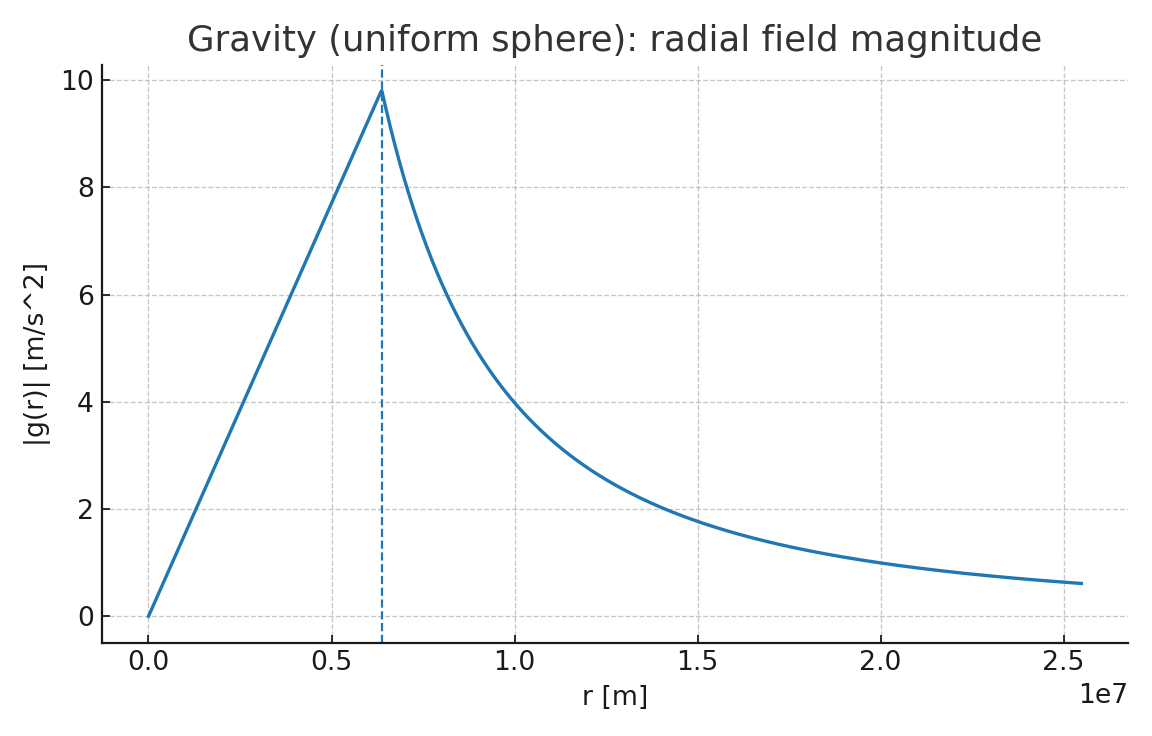
\includegraphics[width=\linewidth]{gravity_vr_profile.png}
    \caption{Radial profile $v_r(r)$ (representative stack).}
    \label{fig:grav:vr}
  \end{subfigure}\hfill
  \begin{subfigure}[t]{0.49\linewidth}
    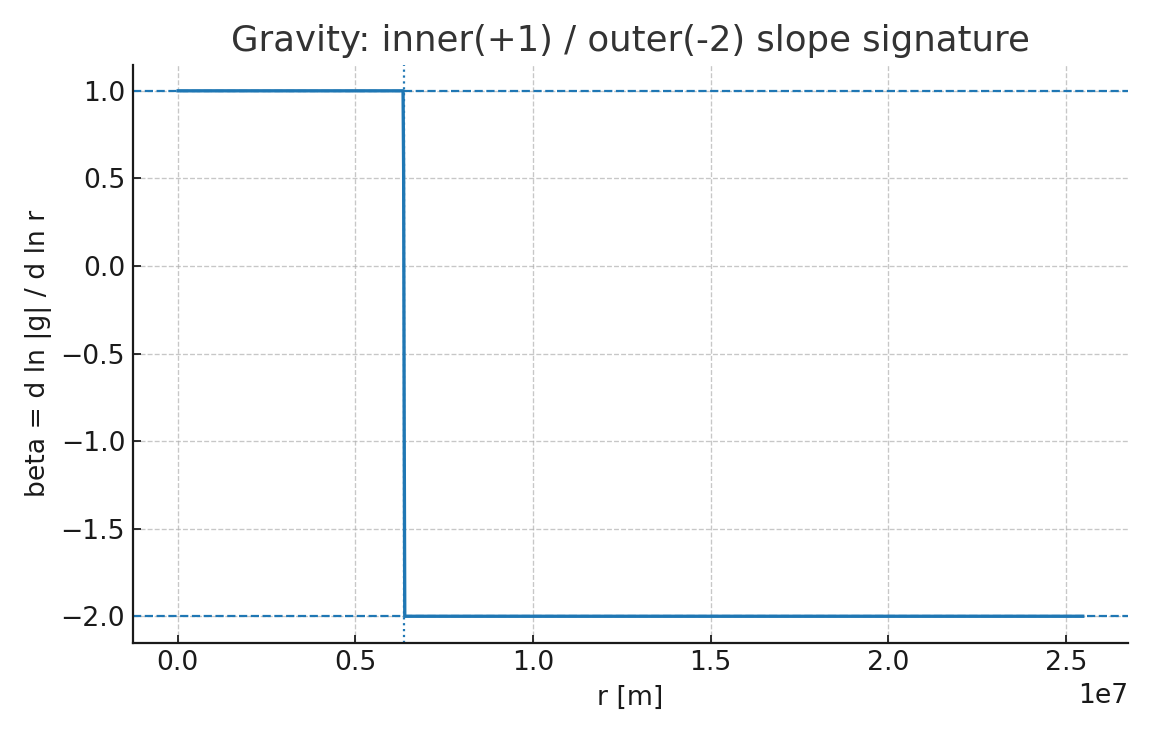
\includegraphics[width=\linewidth]{gravity_beta_signature.png}
    \caption{Log-slope $\beta_O(r)$ showing $+1/-2$.}
    \label{fig:grav:beta}
  \end{subfigure}

  \vspace{0.6em}
  \begin{subfigure}[t]{0.49\linewidth}
    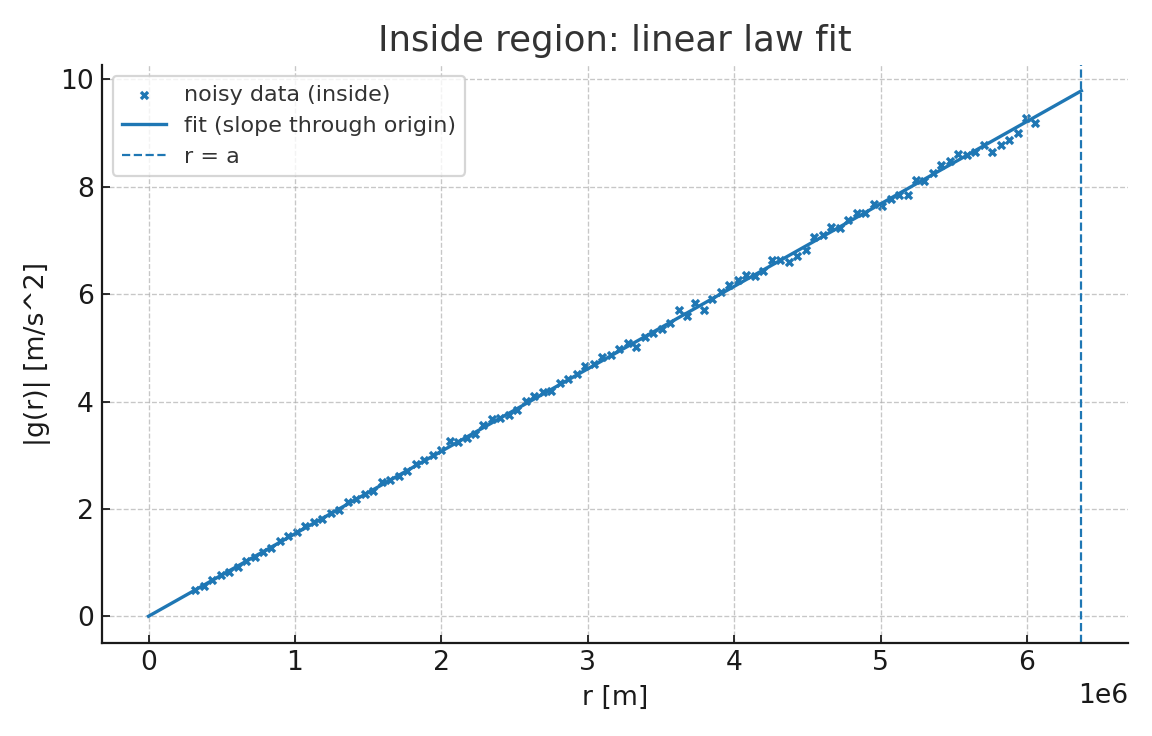
\includegraphics[width=\linewidth]{gravity_inside_fit.png}
    \caption{Interior fit $\;v_r=s_{\rm in}\,r\;$ (through origin).}
    \label{fig:grav:inside}
  \end{subfigure}\hfill
  \begin{subfigure}[t]{0.49\linewidth}
    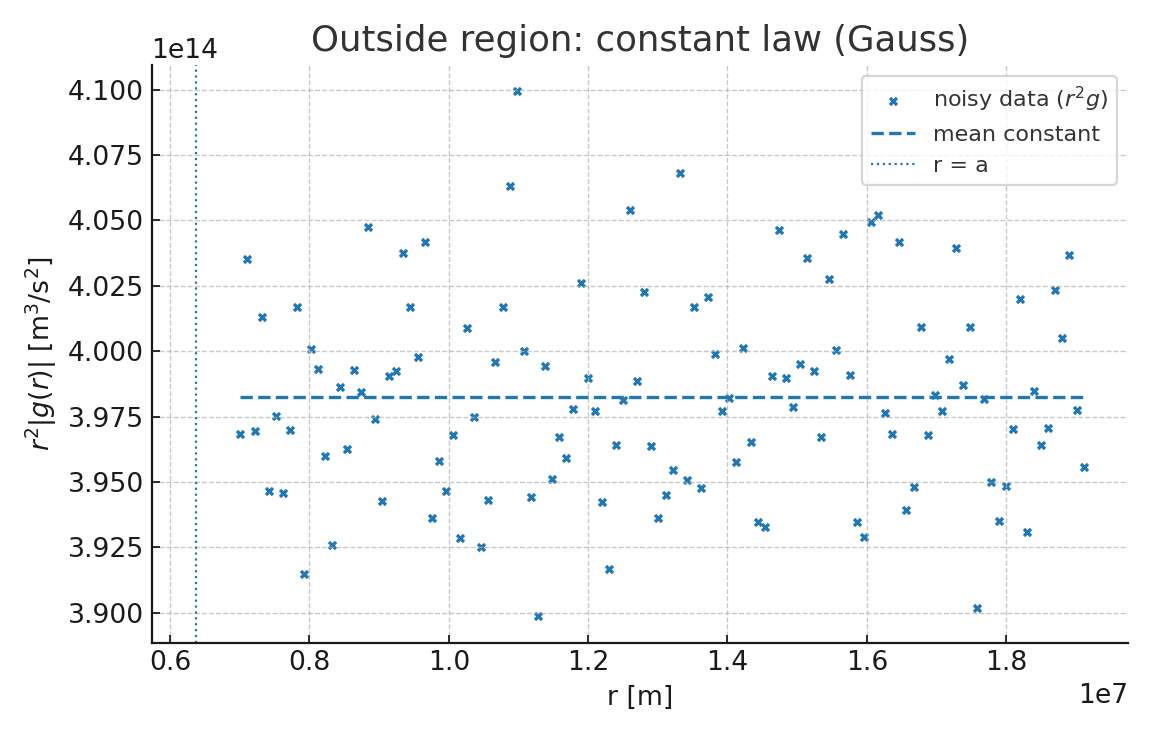
\includegraphics[width=\linewidth]{gravity_outside_constant.png}
    \caption{Exterior Gauss constant $C_{\rm out}=r^2 v_r$.}
    \label{fig:grav:cout}
  \end{subfigure}
\end{figure}

\noindent\textbf{Calibration.} Coupling via counts: compare $G_{\rm in}\propto s_{\rm in}/\rho_N$ and $G_{\rm out}\propto C_{\rm out}/N$; report weighted $G^*$.
\addfig{gravity_G_estimates.png}{Gravity avatar calibration from interior/exterior pulls.}{fig:grav:G}

\chapter{Benchmark II: Electrostatics ⇒ Same Role Signature}
\section*{Plain-language overview}
Replacing masses by charges and $G$ by $1/4\pi\varepsilon_0$ yields the same T1 geometry.

\begin{figure}[htbp]\centering
  \begin{subfigure}[t]{0.49\linewidth}
    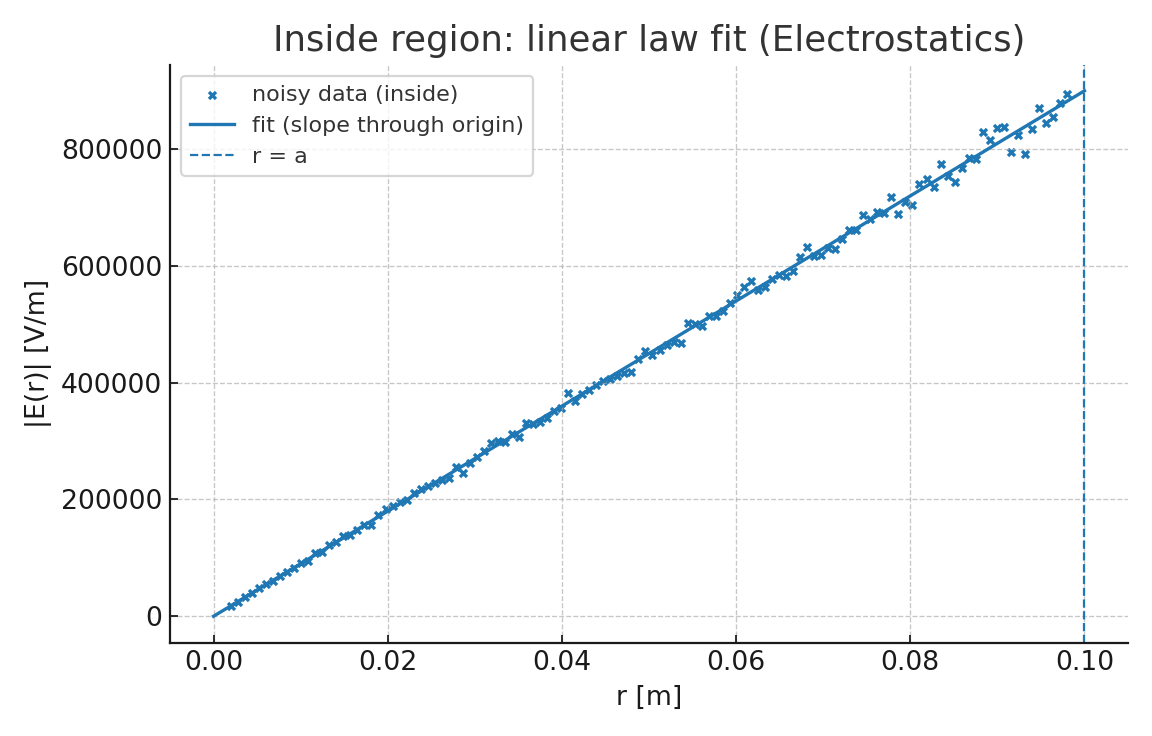
\includegraphics[width=\linewidth]{electrostatics_inside_fit.png}
    \caption{Interior linear rise ($+1$).}
    \label{fig:em:inside}
  \end{subfigure}\hfill
  \begin{subfigure}[t]{0.49\linewidth}
    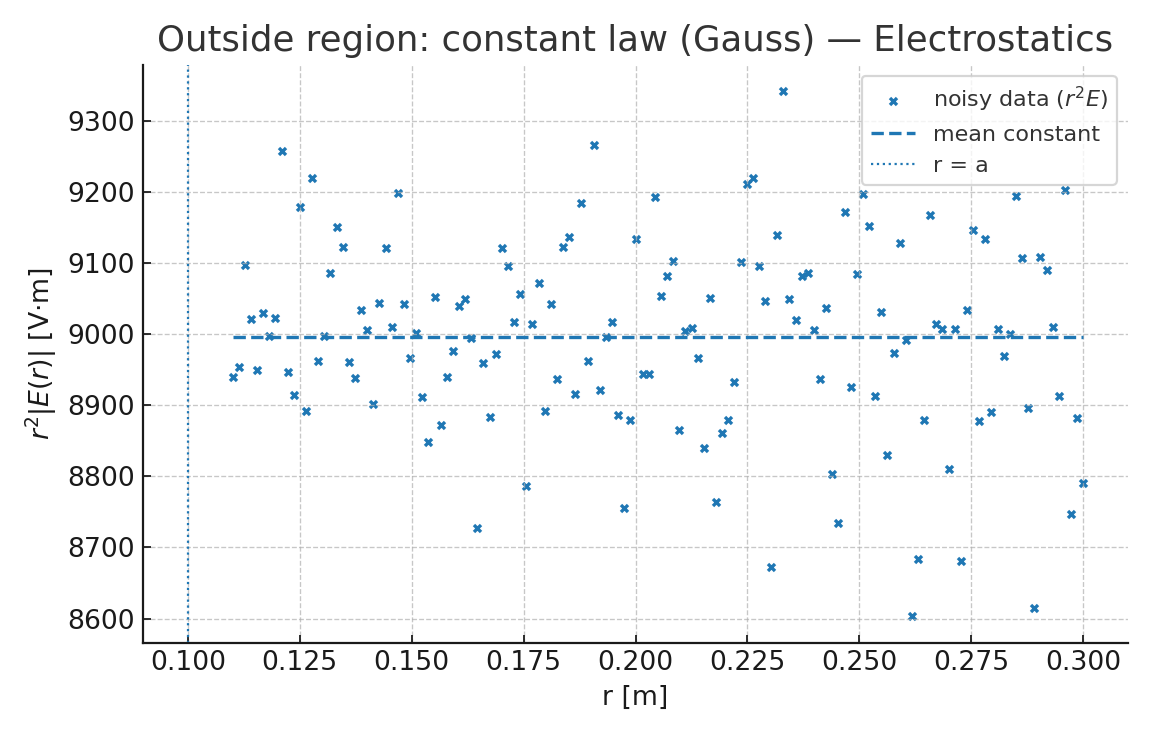
\includegraphics[width=\linewidth]{electrostatics_outside_constant.png}
    \caption{Exterior Gauss constant ($-2$ slope).}
    \label{fig:em:cout}
  \end{subfigure}

  \vspace{0.6em}
  \begin{subfigure}[t]{0.49\linewidth}
    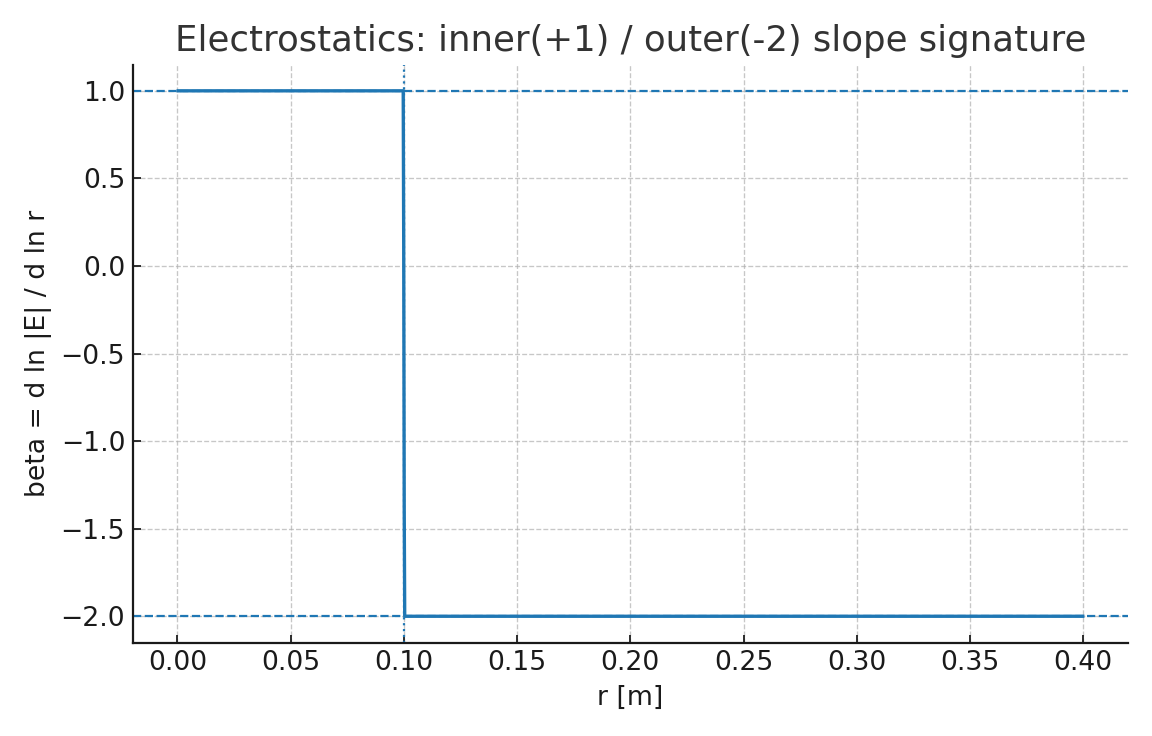
\includegraphics[width=\linewidth]{electrostatics_beta_signature.png}
    \caption{Slope $\beta_O(r)$ reproduces $+1/-2$.}
    \label{fig:em:beta}
  \end{subfigure}\hfill
  \begin{subfigure}[t]{0.49\linewidth}
    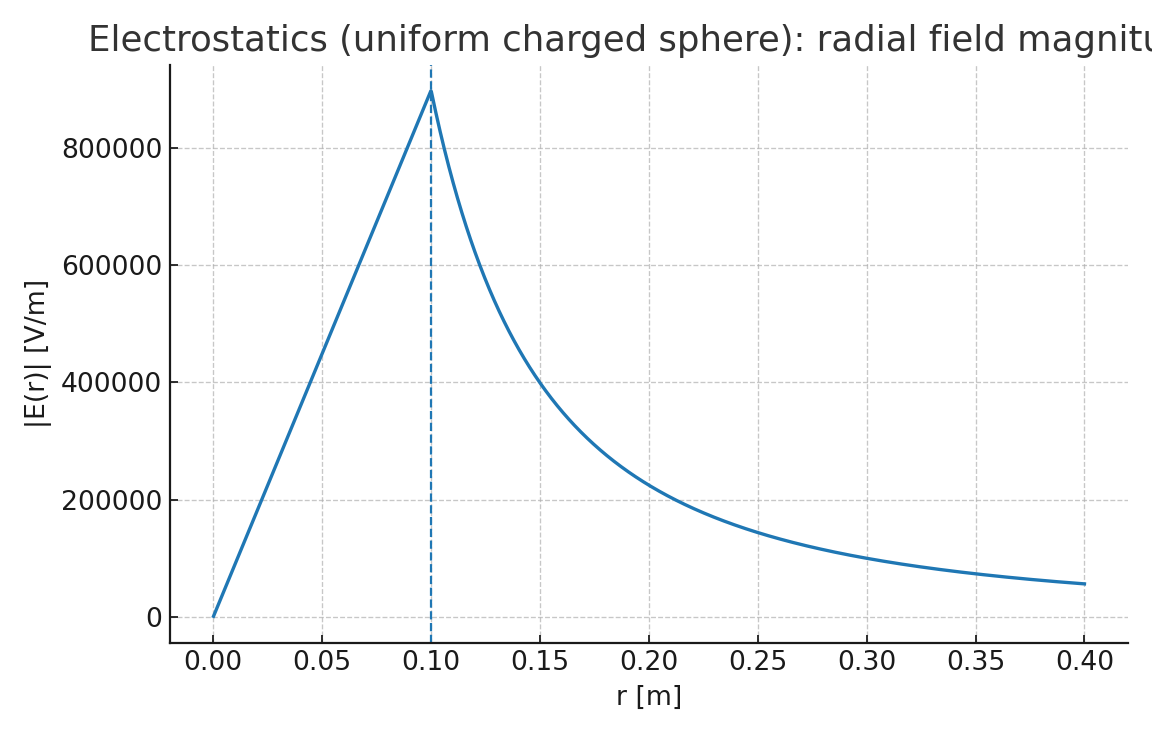
\includegraphics[width=\linewidth]{electrostatics_Emag_profile.png}
    \caption{Field magnitude profile $E(r)$.}
    \label{fig:em:Emag}
  \end{subfigure}
\end{figure}

\addfig{electrostatics_param_estimates.png}{Electrostatics avatar: parameter checks vs.\ counts.}{fig:em:params}

\chapter{Benchmark III: Carrier vs.\ Imprint (Payload/Flux Families)}
\section*{Plain-language overview}
The carrier is $O$-driven (guidance), while binding shells $b(r)$ imprint shape (emission/attenuation). Profiles separate cleanly into carrier asymptotes and environment-dependent imprints.

\begin{figure}[htbp]\centering
  \begin{subfigure}[t]{0.49\linewidth}
    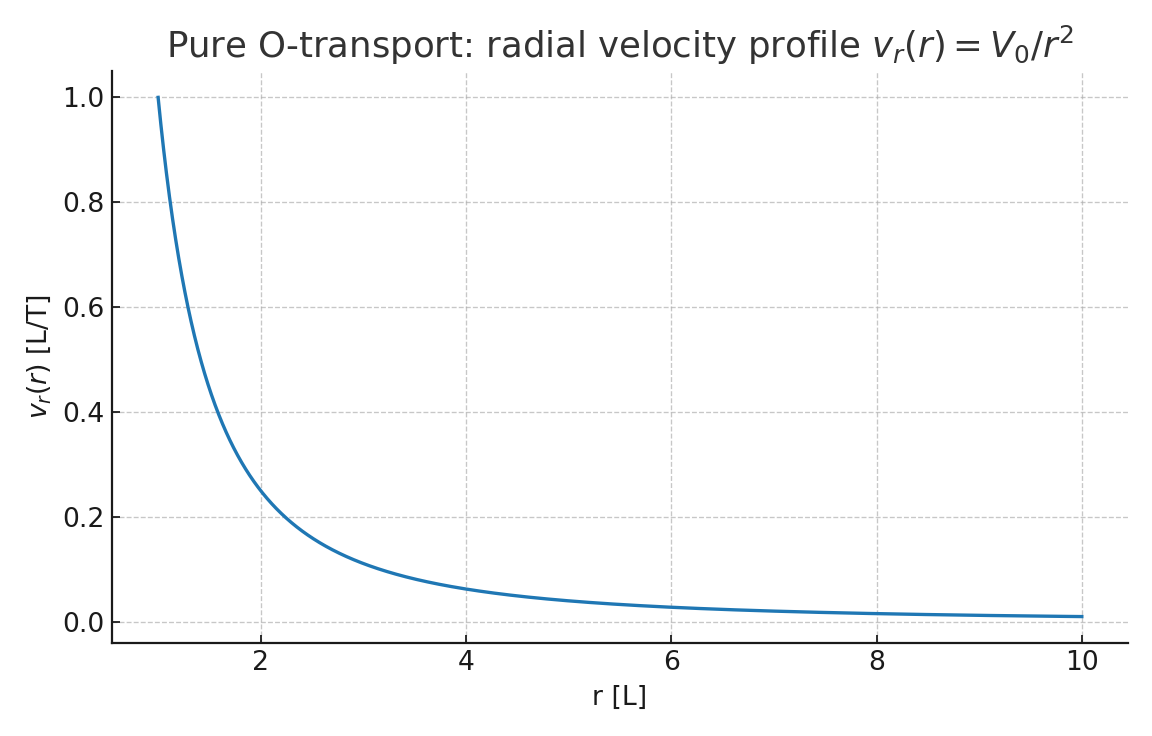
\includegraphics[width=\linewidth]{Otransport_vr_profile.png}
    \caption{$O$-transport carrier: $v_r(r)$ archetype.}
    \label{fig:carrier:vr}
  \end{subfigure}\hfill
  \begin{subfigure}[t]{0.49\linewidth}
    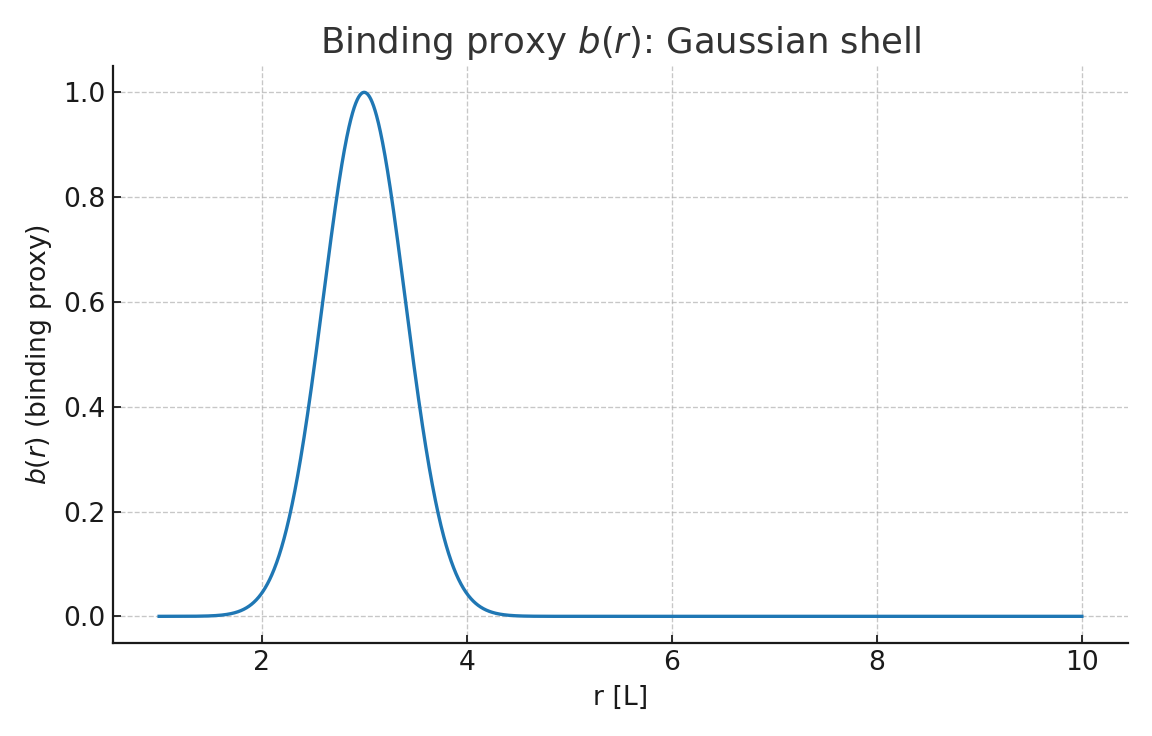
\includegraphics[width=\linewidth]{binding_proxy_shell.png}
    \caption{Binding proxy $b(r)$ (imprint shell).}
    \label{fig:carrier:b}
  \end{subfigure}

  \vspace{0.6em}
  \begin{subfigure}[t]{0.49\linewidth}
    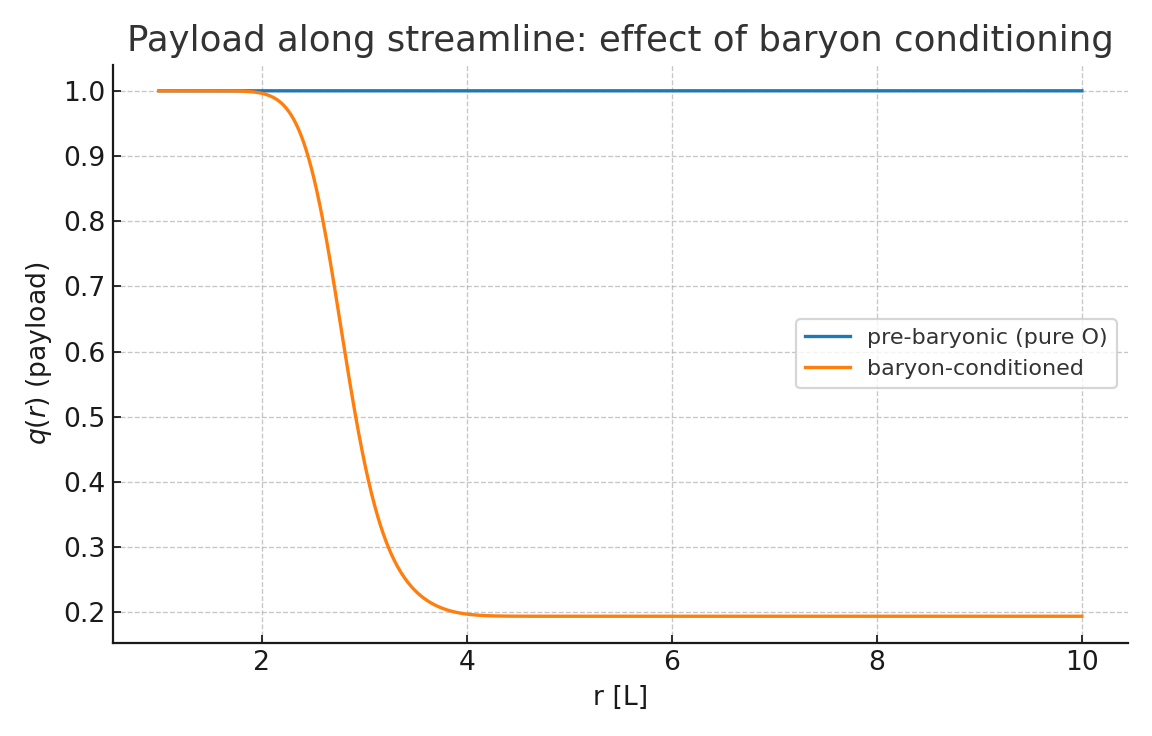
\includegraphics[width=\linewidth]{payload_profiles.png}
    \caption{Payload families $q(r)$ under different $b(r)$.}
    \label{fig:carrier:payload}
  \end{subfigure}\hfill
  \begin{subfigure}[t]{0.49\linewidth}
    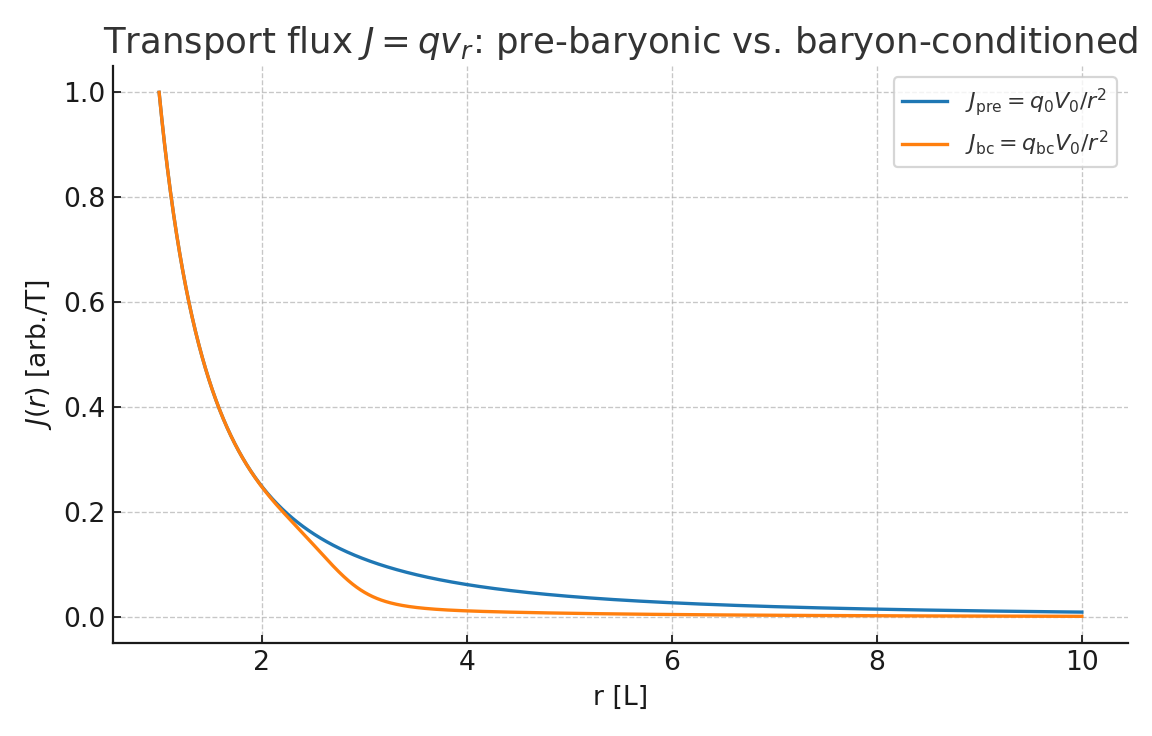
\includegraphics[width=\linewidth]{flux_profiles.png}
    \caption{Flux families $J(r)$; same carrier asymptote.}
    \label{fig:carrier:flux}
  \end{subfigure}
\end{figure}

\begin{figure}[htbp]\centering
  \begin{subfigure}[t]{0.49\linewidth}
    \includegraphics[width=\linewidth]{realism_vr_profile.png}
    \caption{Realistic composite: observed $v_r(r)$.}
    \label{fig:real:vr}
  \end{subfigure}\hfill
  \begin{subfigure}[t]{0.49\linewidth}
    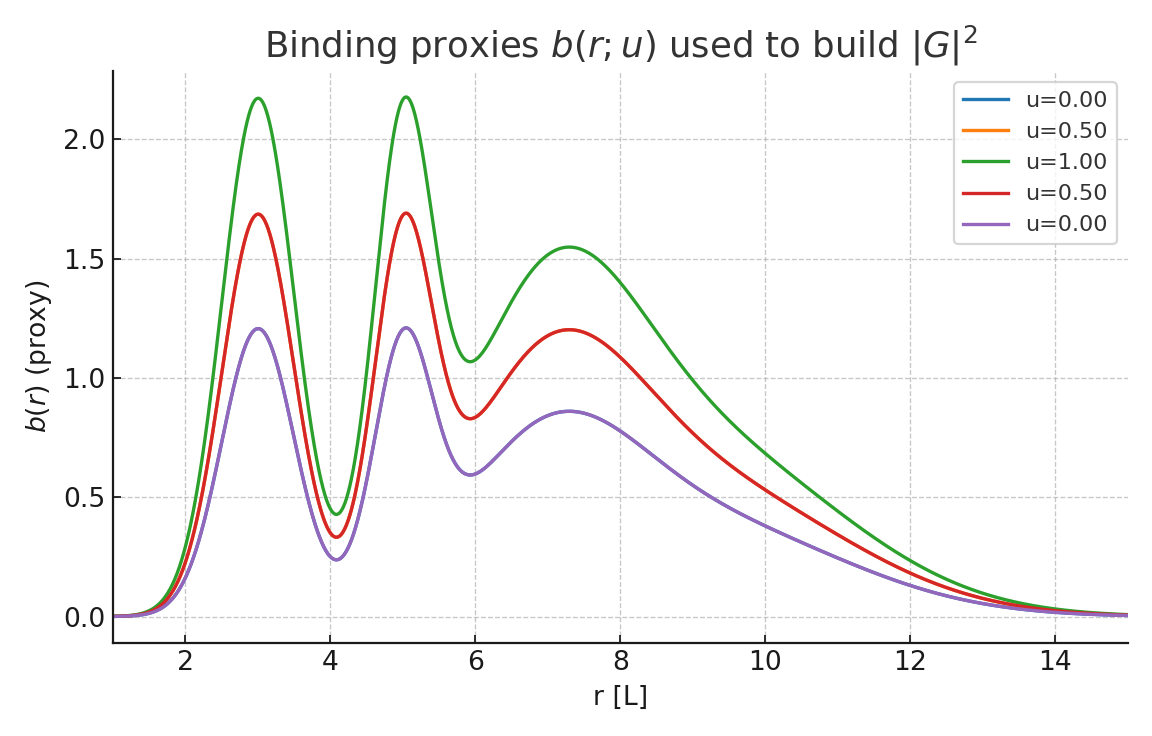
\includegraphics[width=\linewidth]{realism_b_profiles.png}
    \caption{Realistic $b(r)$ envelopes (imprint diversity).}
    \label{fig:real:b}
  \end{subfigure}
\end{figure}

\chapter{Benchmark IV: Sensitivity to Source/Sink Knobs}
\section*{Plain-language overview}
One-at-a-time scans expose which parameters control shape vs.\ amplitude.

\begin{figure}[htbp]\centering
  \begin{subfigure}[t]{0.49\linewidth}
    \includegraphics[width=\linewidth]{sensitivity_q_mu0.png}
    \caption{Sensitivity in $\mu$ (near/far-field impact).}
    \label{fig:sens:mu}
  \end{subfigure}\hfill
  \begin{subfigure}[t]{0.49\linewidth}
    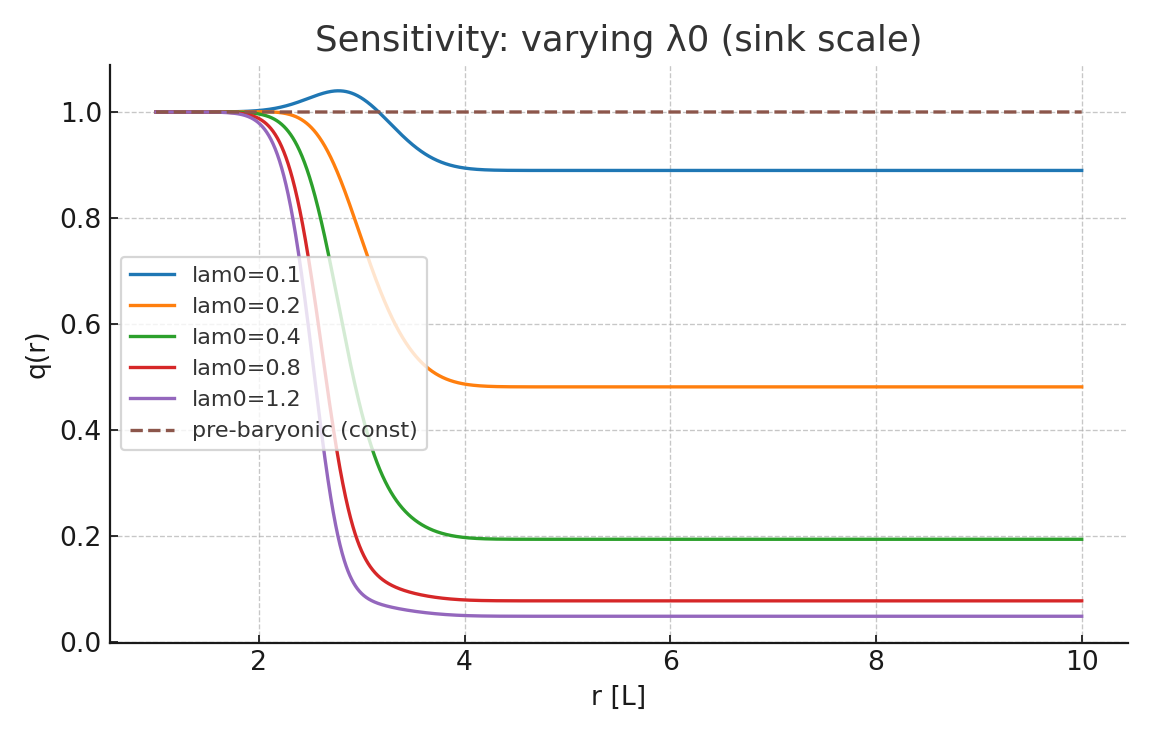
\includegraphics[width=\linewidth]{sensitivity_q_lam0.png}
    \caption{Sensitivity in $\lambda$ (damping/attenuation).}
    \label{fig:sens:lam}
  \end{subfigure}
\end{figure}

\chapter{Benchmark V: Thresholds and Hysteresis (T3)}
\section*{Plain-language overview}
Control sweeps reveal nucleation and persistence; loop area $\mathcal A_{\rm loop}$ quantifies feedback.

\begin{figure}[htbp]\centering
  \begin{subfigure}[t]{0.49\linewidth}
    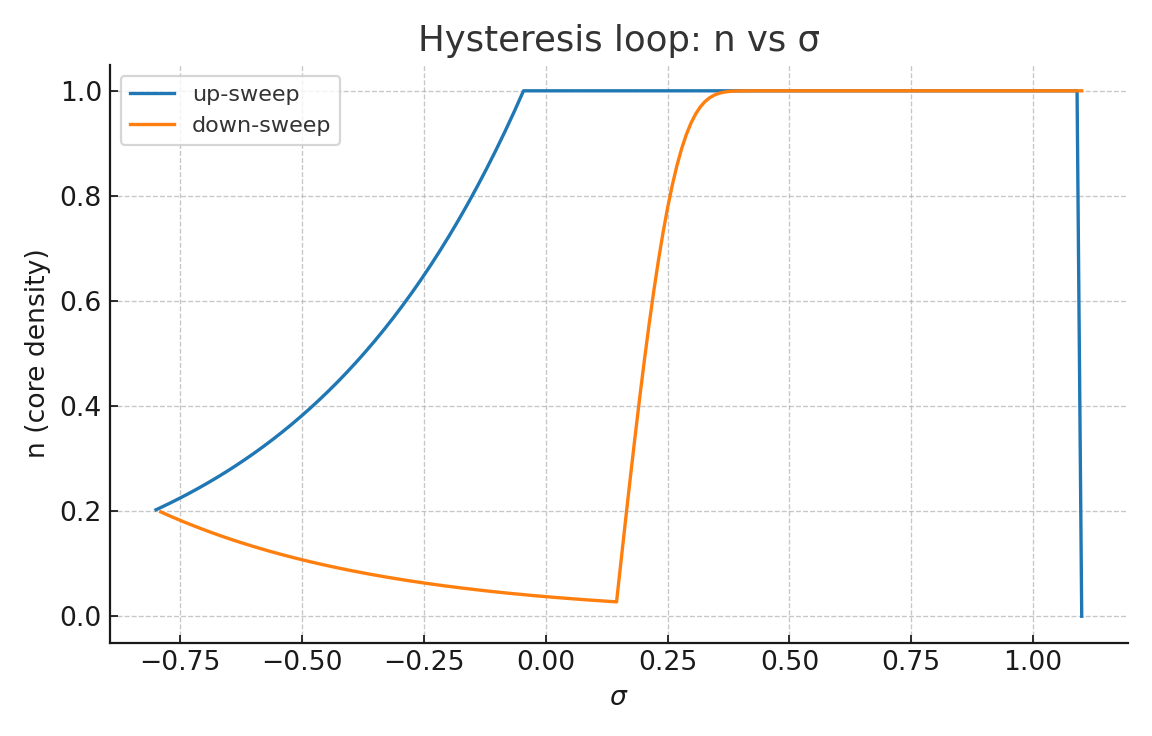
\includegraphics[width=\linewidth]{hysteresis_n_vs_sigma.png}
    \caption{Canonical loop: $n$ vs.\ role-intensity $\sigma$.}
    \label{fig:hyst:canon}
  \end{subfigure}\hfill
  \begin{subfigure}[t]{0.49\linewidth}
    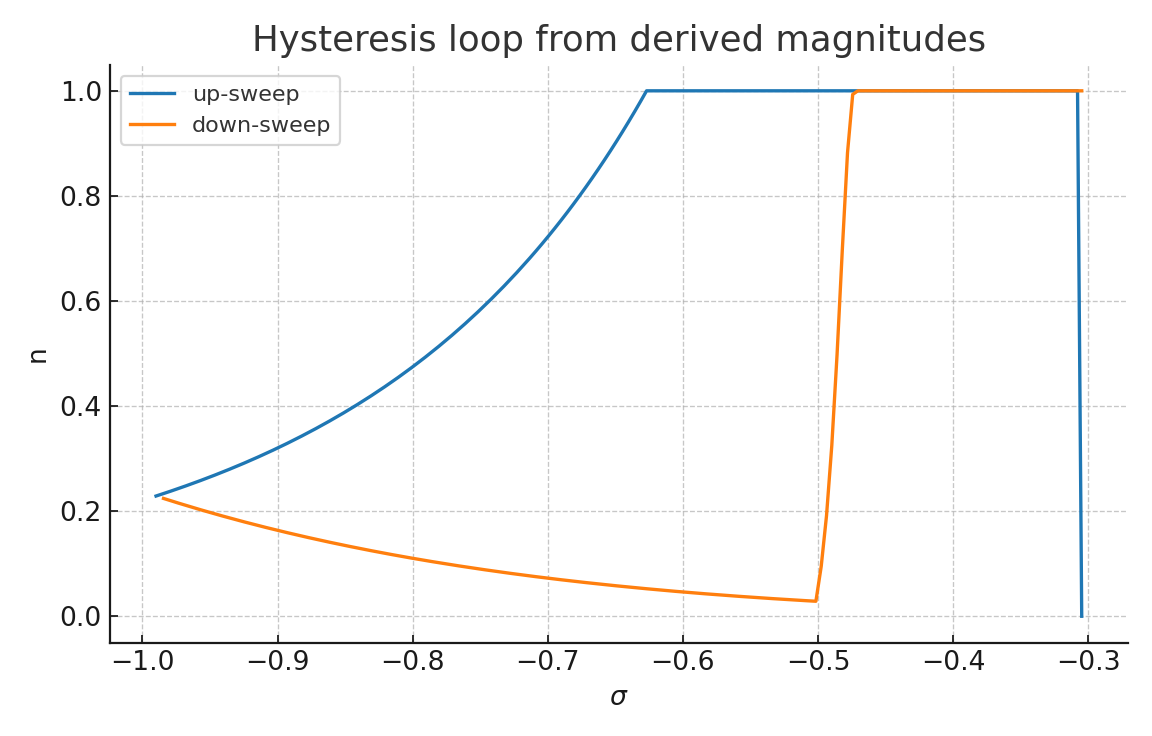
\includegraphics[width=\linewidth]{realism_hysteresis_n_sigma.png}
    \caption{Realistic loop under noise/conditioning.}
    \label{fig:hyst:real}
  \end{subfigure}
\end{figure}

\chapter{Benchmark VI: BH-Prox Signatures (Role View)}
\section*{Plain-language overview}
Near compact objects, the same role logic splits carrier vs.\ imprint; thresholds appear as intensity transitions.

\begin{figure}[htbp]\centering
  \begin{subfigure}[t]{0.49\linewidth}
    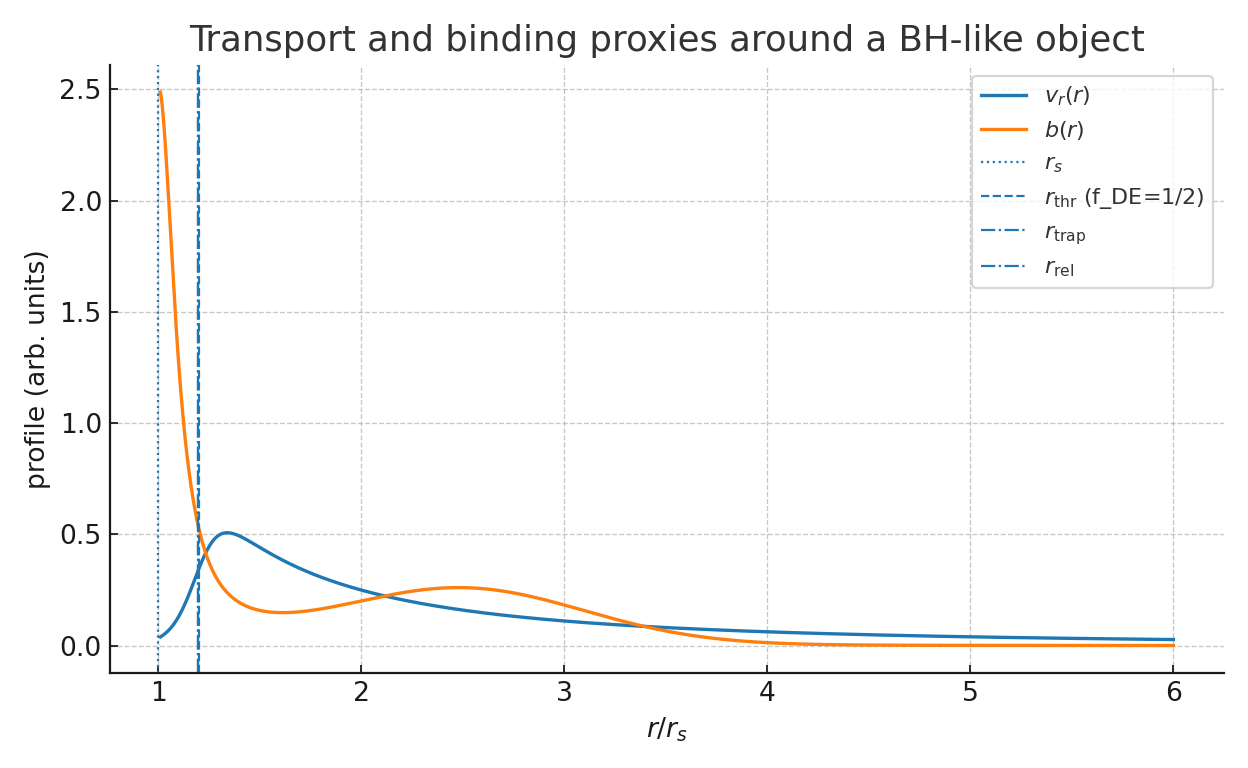
\includegraphics[width=\linewidth]{bh_profiles_vr_b.png}
    \caption{Carrier $v_r$ with binding proxy $b(r)$ (BH-prox).}
    \label{fig:bh:profiles}
  \end{subfigure}\hfill
  \begin{subfigure}[t]{0.49\linewidth}
    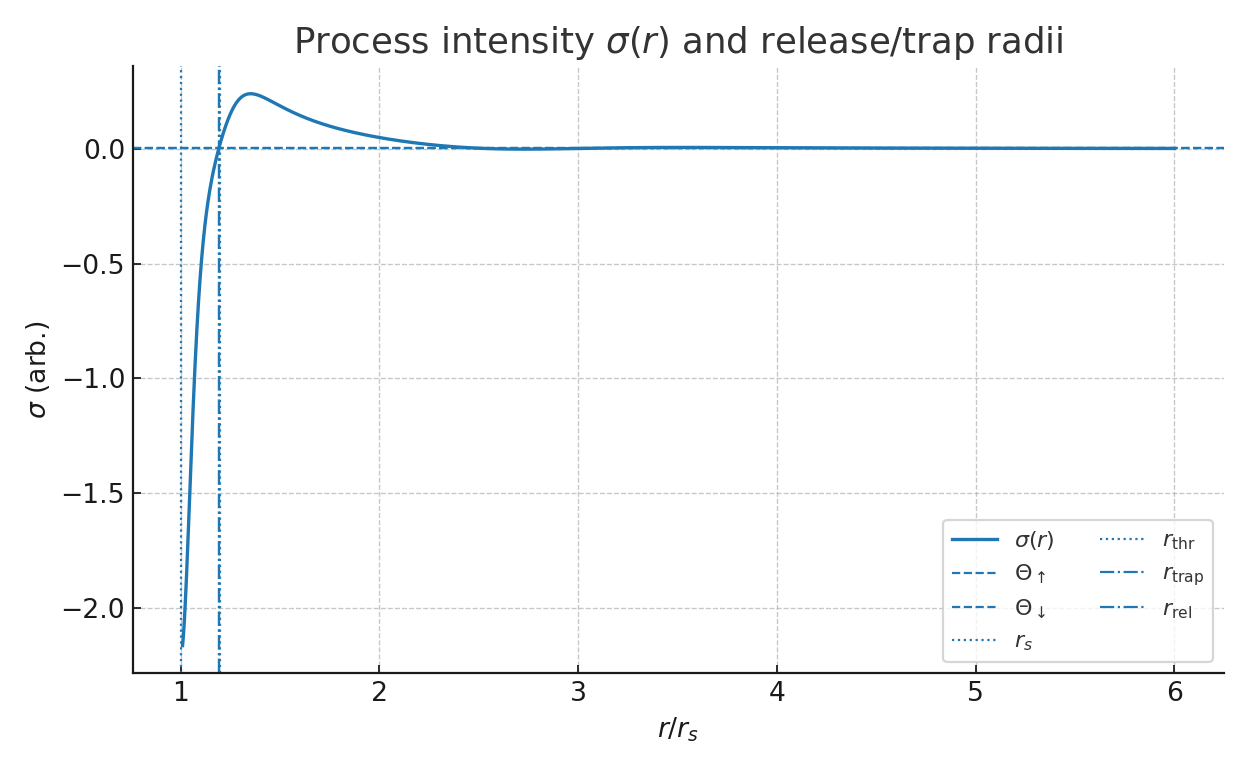
\includegraphics[width=\linewidth]{bh_sigma_thresholds.png}
    \caption{Role-intensity $\sigma$ thresholds around horizon.}
    \label{fig:bh:sigma}
  \end{subfigure}
\end{figure}

\section*{Protocol}
Sweep a control (e.g., density, field strength, feed); record the order parameter; extract $(\Theta_\uparrow,\Theta_\downarrow)$ and loop area $\mathcal A_{\rm loop}$.

\section*{Nulls}
Shuffle control labels across runs; time-reversal surrogates for the sweep; pipeline splits.

\section*{Report}
Thresholds with CIs, loop areas, dwell time $T_{\rm above}$, and window validity ($\Delta f\le 1/W$).

\addfig{figures/hysteresis.png}{Thresholds and hysteresis: $\sigma$ vs.\ control, nucleation/persistence loop in $n(\sigma)$.}{fig:res:hysteresis}[0.9]

% ---- Compact calibration & standards page ----
\chapter*{Minimal Calibration \& Reporting Standard}
\noindent\textbf{Core metrics.}
\begin{itemize}\setlength\itemsep{0.2em}
\item \textbf{T1 (Orientation)}: inner/exterior slopes (3D: $+1/-2$); identity residual $\delta_I=\big|\Cout/\sinIn-a^3\big|/a^3$; sector avatar ($G$, $1/4\pi\varepsilon_0$) cross-check.
\item \textbf{Carrier–Imprint}: carrier exponents vs.\ imprint parameters $b(r)$; stability across environments.
\item \textbf{T3 (Hysteresis)}: $(\Theta_\uparrow,\Theta_\downarrow)$, loop area $\mathcal A_{\rm loop}>0$, dwell $T_{\rm above}$.
\end{itemize}

\noindent\textbf{Nulls and robustness.}
Label/shell shuffles (stacks), phase/surrogate shuffles (spectra/time series), degree-preserving graph shuffles (networks), independent pipeline splits. Target $p<0.01$ for null rejection. Report bootstrap/jackknife confidence bands.

\noindent\textbf{Window validity and disclosure.}
State window constraints ($\Delta f\le1/W$ for dwell-type measures), selection/mask transfer functions, and provide brief code/recipe notes for external replication.

\chapter*{Test ID Map (for inline boxes)}
\begin{tabular}{@{}ll@{}}
\toprule
ID & Where used (examples) \\
\midrule
\textbf{T1} & Orientation identity in stacks (Bench.~I–II; Parts I, III, IV) \\
\textbf{Carrier–Imprint} & Radiation profiles with $b(r)$ shaping (Bench.~III; Part II) \\
\textbf{Sensitivity} & Shape vs.\ amplitude controls (Bench.~IV; Parts II–IV) \\
\textbf{Stacking} & Ensemble vs.\ representative profiles (Bench.~V; Parts III–IV) \\
\textbf{T3} & Thresholds, hysteresis, dwell (Bench.~VI; Parts II, IV–V, VII) \\
\bottomrule
\end{tabular}

\appendix

\chapter{Symbols, Units, and Notation}\label{app:symbols}
\begin{table}[htbp]\centering
\caption{Core symbols, units, and role mapping (orientation/binding/counting).}
\begin{tabular}{llp{0.58\linewidth}}\toprule
Symbol & Units & Meaning \\ \midrule
$S,N$ & – & Basis states (substrate $S$ / contrast $N$) on Ur-fabric.\\
$C$ & – & Diagnostic counting (non-operative); reads real overlap events.\\
$O,G$ & sector-dep. & Roles: guidance/transport $O$, binding/structuring $G$.\\
$K:=O\!\circ G$ & – & Overlap composition (“flow meets knot”), order matters.\\
$\tau^O,\ \tau^K$ & counts & Process clocks (event counters) for $O$- and $K$-events.\\
$t:=C[\tau^K]$ & time & Coarse-grained continuation of counted $K$-events.\\
$\mathbf v_O$ & sector-dep. & Orientation field (e.g.\ $g$ in gravity, $\mathbf E$ in EM).\\
$\kappa_O$ & sector-dep. & Orientation coupling; avatars: $\kappa_O^{(\mathrm{grav})}=G$, $\kappa_O^{(\mathrm{EM})}=1/4\pi\varepsilon_0$.\\
$\Omega$ & sector-dep. & Orientation potential; $\mathbf v_O=\kappa_O\nabla\Omega$.\\
$\rho_N$ & sector-dep. & Deficit density (source of $\Omega$ in weak field).\\
$a$ & L & Core radius / stacking scale.\\
$s_{\rm in}$ & field/L & Inner radial slope $dv_r/dr$ at $r\le a$.\\
$C_{\rm out}$ & field$\cdot$L$^{D-1}$ & Gauss constant $r^{D-1}v_r$ at $r\ge a$ (in $D$ dims).\\
$D$ & – & Spatial dimension (default $D=3$).\\
$b(r)$ & – & Binding shell/profile (imprint).\\
$\Theta,\ \sigma_c$ & role-intensity & Systemic seed threshold / critical persistence threshold.\\
$\Lambda$ & 1/time & Effective loss/degradation rate.\\
$W$ & time & Window length (conditions dwell).\\
$T_{\rm above}$ & time & Time spent above threshold (plateau dwell).\\
$\mathrm{SEC}$ & – & Existential stability proxy $\propto \frac{\tau^K}{S+N}\cdot\frac{T_{\rm above}}{W}$.\\
$R_{\rm tick}$ & – & Tick-rate ratio $f_{\rm agent}/f_{\rm env}$.\\
$R_0$ & – & Autarky ratio (self-output / self-needs).\\
$C_1(k)$ & [0,1] & Cross-coherence (flow-like vs.\ potential-like field).\\
$C_2$ & [0,1] & Structure–flow coordination (spectral or info-theoretic).\\
$\mathcal A_{\rm loop}$ & area & Hysteresis loop area (on/off asymmetry).\\
$G_{\rm st}$ & – & Structural/binding graph (molecules, brain, systems).\\
$\mathbf J$ & sector-dep. & Flow vector (currents/fluxes/activations).\\
$L(\cdot)$ & – & Graph Laplacian; leading mode(s) $\mathbf u$.\\
\bottomrule
\end{tabular}
\end{table}

\chapter{Time and Clocks: Definitions and Constraints}\label{app:time}
\section*{Definitions}
\begin{align}
\tau^O &:= \operatorname{ord}\{O_k\}\quad\text{(counts guidance events)},\\
\tau^K &:= \operatorname{ord}\{K_k\},\ \ K:=O\!\circ G\quad\text{(counts overlap events)},\\
t &:= C[\tau^K]\quad\text{(coarse-grained continuation; diagnostic, non-operative).}
\end{align}

\paragraph{Window validity (dwell-type measures).}
For any metric derived from plateau dwell $T_{\rm above}$ over window $W$,
\[
\Delta f \le \frac{1}{W}
\]
must hold for spectral/temporal estimates to be meaningful (report $\Delta f$ and $W$).

\chapter{Orientation Identity: Short Derivation (T1) and $D$-Generalization}\label{app:T1}
\section*{Weak-field in $D$ dimensions}
Assume $\mathbf v_O=\kappa_O\nabla\Omega$ and $\nabla\!\cdot\mathbf v_O=S_D\,\kappa_O\,\rho_N$, with $S_D$ a geometric constant. For a spherically symmetric core of radius $a$ with constant $\rho_N$ inside and $0$ outside:
\begin{enumerate}
\item \textbf{Exterior ($r\ge a$):} Gauss counting gives $r^{D-1}v_r=C_{\rm out}$ (constant) $\Rightarrow$ $v_r\propto r^{-(D-1)}$ (slope $-(D-1)$).
\item \textbf{Interior ($r\le a$):} Regularity requires $v_r\propto r$ (slope $+1$), hence $v_r=s_{\rm in}\,r$.
\end{enumerate}
Matching at $r=a$ yields the parameter-free identity
\[
\boxed{~\frac{C_{\rm out}}{s_{\rm in}}=a^{D}~}\,,
\]
which reduces in $D=3$ to $C_{\rm out}/s_{\rm in}=a^3$ and exterior slope $-2$.

\paragraph{Calibration avatars.}
Gravity: $v_O\leftrightarrow g$, $\kappa_O^{(\mathrm{grav})}=G$. \quad
Electrostatics: $v_O\leftrightarrow E$, $\kappa_O^{(\mathrm{EM})}=1/(4\pi\varepsilon_0)$.

\chapter{Measurement Standards and Null Tests (Expanded)}\label{app:standards}
\section*{Global principles}
\begin{itemize}
\item \textbf{Declare metrics a priori:} T1 slopes \& identity residual $\delta_I$, $C_1(k)$ band center/width, $C_2$ plateaus ($T_{\rm above}$, $\mathcal A_{\rm loop}$), thresholds $(\Theta_\uparrow,\Theta_\downarrow)$.
\item \textbf{Window validity:} report $(W,\Delta f)$; ensure $\Delta f\le 1/W$.
\item \textbf{Uncertainties:} provide bootstrap/jackknife confidence bands; show sensitivity to selection/masks.
\item \textbf{Independent pipelines:} at least one full re-implementation or method split (e.g.\ TE vs.\ Granger; alternative stackers).
\end{itemize}

\section*{Null-test catalogue}
\begin{enumerate}
\item \textbf{Label shuffles (stacks):} randomize object–bin assignments; recompute T1.
\item \textbf{Shell randomization (radial):} randomize annulus ordering while keeping counts.
\item \textbf{Phase-preserving surrogates:} IAAFT/phase-shuffle for spectra/time series; test $C_1(k)$ band collapse.
\item \textbf{Graph-preserving shuffles:} degree-preserving rewires for $G_{\rm st}$ before $C_2$.
\item \textbf{Pipeline splits:} alternative estimators, masks, or calibration sources; compare within tolerance.
\end{enumerate}
\emph{Target:} reject nulls at $p<0.01$ for claimed bands/plateaus.

\section*{Stacking standard (T1)}
\begin{enumerate}
\item Bin by effective radius $a$; estimate $s_{\rm in}$ (regression through origin) and $C_{\rm out}$ (constancy of $r^{D-1}v_r$).
\item Report slopes with CIs; compute $\delta_I=\big|C_{\rm out}/s_{\rm in}-a^D\big|/a^D$.
\item Run label/shell shuffles; include bootstrap bands and pipeline split comparison.
\end{enumerate}

\section*{Cross-coherence standard ($C_1$)}
\begin{enumerate}
\item Register flow-like $X$ and potential-like $Y$ to a common grid/mask; deconvolve windows.
\item Compute $P_{XX},P_{YY},P_{XY}$ and $C_1(k)=|P_{XY}|/\sqrt{P_{XX}P_{YY}}$.
\item Phase-shuffle $Y$ (keep amplitude) $\Rightarrow$ band must vanish ($p<0.01$).
\end{enumerate}

\section*{Hysteresis/plateau standard (T3)}
\begin{enumerate}
\item Sweep a control (feed, field, load); compute an order metric (e.g.\ occupancy, flux, $C_2$).
\item Extract $(\Theta_\uparrow,\Theta_\downarrow)$ and loop area $\mathcal A_{\rm loop}$; report $T_{\rm above}$.
\item Use time-reversal surrogates and label shuffles; ensure window validity.
\end{enumerate}

\chapter{Computation Recipes (No-Surprise Implementations)}\label{app:recipes}
\section*{Cross-coherence $C_1(k)$}
\begin{enumerate}
\item Preprocess $X,Y$ (demean, window, common mask); FFT on equal grids.
\item Estimate spectra: $P_{XX},P_{YY}$; cross-spectrum $P_{XY}$ with taper averaging.
\item Form $C_1(k)$; bootstrap over segments; \emph{null}: phase-shuffle $Y$ and recompute.
\end{enumerate}

\section*{Coordination $C_2$ (spectral)}
\begin{enumerate}
\item Build $G_{\rm st}$; compute Laplacian $L$ and leading mode(s) $\mathbf u$.
\item Estimate directed flows $\mathbf J$ (e.g.\ Granger/TE/phase-slope index) on matched windows.
\item Compute $C_2=|\mathbf u^\top\mathbf J|/(\|\mathbf u\|\|\mathbf J\|)$; detect plateaus by run-length above a preset quantile.
\end{enumerate}
\emph{Alternative:} information-theoretic $C_2$ by mean TE over edges, normalized to $[0,1]$.

\section*{Plateau and hysteresis detection}
\begin{enumerate}
\item Define threshold $\theta$ as a robust quantile of the metric; plateaus are contiguous runs above $\theta$ (report $T_{\rm above}$).
\item For hysteresis, record metric vs.\ control on up/down sweeps; compute loop area $\mathcal A_{\rm loop}$ (Shoelace formula on the parametric curve).
\end{enumerate}

\chapter{Reporting Templates}\label{app:report}
\section*{Minimal reproducibility checklist}
\begin{enumerate}
\item Metrics declared a priori (T1/T2/T3, thresholds, bands, plateaus).
\item Window validity: $(W,\Delta f)$ reported; selection/mask transfer functions described.
\item Nulls: which, how many, $p$-values; bootstrap/jackknife bands.
\item Independent pipeline description and agreement bounds.
\item Code/recipe notes: versions, seeds, parameter grids.
\end{enumerate}

\section*{Result table skeletons}
\begin{table}[htbp]\centering
\caption{T1 (Orientation) summary by stack bin.}
\begin{tabular}{llllll}\toprule
Bin $a$ & $s_{\rm in}$ & $C_{\rm out}$ & $\delta_I$ & inner/outer slopes & Notes \\\midrule
... & ... & ... & ... & $+1 / -2$ & ...\\ \bottomrule
\end{tabular}
\end{table}

\begin{table}[htbp]\centering
\caption{$C_1(k)$ band summary.}
\begin{tabular}{lllll}\toprule
Band center $k_\star$ & Width $\Delta k$ & $C_{1,\max}$ & Null $p$-value & Splits passed \\\midrule
... & ... & ... & ... & ...\\ \bottomrule
\end{tabular}
\end{table}

\begin{table}[htbp]\centering
\caption{Hysteresis/Plateau summary (T3).}
\begin{tabular}{lllll}\toprule
$\Theta_\uparrow$ & $\Theta_\downarrow$ & $\mathcal A_{\rm loop}$ & $T_{\rm above}$ & Window $(W,\Delta f)$ \\\midrule
... & ... & ... & ... & ...\\ \bottomrule
\end{tabular}
\end{table}

\chapter{Scope, Assumptions, and Limitations}\label{app:limits}
\begin{itemize}
\item \textbf{Weak-field avatar:} T1 holds under locality, isotropy, linear superposition; strong non-linearities require sector models (but T1 provides a null-benchmark).
\item \textbf{Diagnostics, not forces:} $C$ never acts on states; it only counts overlaps. Coherences ($C_0,C_1,C_2$) are measurement-grade summaries.
\item \textbf{Universality stance:} roles $O,G$ are primitive on Ur-fabric; higher layers use effective avatars $O_{\rm eff},G_{\rm eff}$ with renormalized couplings; curl/nonlinear corrections vanish in weak field.
\end{itemize}

% =============================
% BACK MATTER
% =============================

% (Optional) Acknowledgments
\chapter*{Acknowledgments}
\addcontentsline{toc}{chapter}{Acknowledgments}
We thank colleagues and readers for discussions and feedback. Any remaining errors are our own.

% (Optional) Data, Code, and Materials Availability
\chapter*{Data, Code, and Materials Availability}
\addcontentsline{toc}{chapter}{Data, Code, and Materials Availability}
All analysis recipes (stacking, $C_1(k)$, $C_2$, hysteresis loops) and plotting scripts are available at: \texttt{<repository or archive link>}. 
Where third-party datasets are used, access instructions and licenses are documented in the repository’s \texttt{README.md}. 
We provide seeds, parameter grids, and exact configuration files for full replication.

% (Optional) Author Contributions (CRediT style)
\chapter*{Author Contributions}
\addcontentsline{toc}{chapter}{Author Contributions}
\textbf{Conceptualization:} A.~Author. \quad
\textbf{Methodology:} A.~Author. \quad
\textbf{Software:} A.~Author. \quad
\textbf{Validation:} A.~Author. \quad
\textbf{Writing—original draft:} A.~Author. \quad
\textbf{Writing—review \& editing:} A.~Author.

% (Optional) Competing Interests
\chapter*{Competing Interests}
\addcontentsline{toc}{chapter}{Competing Interests}
The author declares no competing interests.

% (Optional) Ethical and Safety Considerations
\chapter*{Ethical and Safety Considerations}
\addcontentsline{toc}{chapter}{Ethical and Safety Considerations}
This work proposes measurement-grade diagnostics (e.g., $C_1$, $C_2$, dwell/hysteresis) and reporting standards. 
Domain-specific interventions or human/AI experiments should conform to relevant ethical review processes and safety constraints.

% (Optional) Reproducibility Checklist (short)
\chapter*{Reproducibility Checklist}
\addcontentsline{toc}{chapter}{Reproducibility Checklist}
\begin{itemize}
  \item Metrics declared a priori (T1/T3, $C_1(k)$ band, $C_2$ plateaus, thresholds $(\Theta_\uparrow,\Theta_\downarrow)$).
  \item Window validity reported ($W$, $\Delta f$, mask/selection transfer).
  \item Null tests (label/shell/phase/graph shuffles) with $p$-values; bootstrap/jackknife CIs.
  \item Independent pipeline splits and agreement bounds.
  \item Code, seeds, and parameter grids archived (see Data/Code Availability).
\end{itemize}

% (Optional) How to Cite This Work
\chapter*{How to Cite This Work}
\addcontentsline{toc}{chapter}{How to Cite This Work}
If you reference this manuscript, please cite as:
\begin{quote}
A.~Author. \emph{Thresholds, Coherence, and Emergent Time from Ur-Fabric to Cosmos, Life, and Mind: A Process-Based, Falsifiable Role Calculus}. Year. Version/DOI: \texttt{<doi or URL>}.
\end{quote}
\noindent Bib\LaTeX\ entry (add to \texttt{references.bib}):
\begin{verbatim}
@misc{author_role_calculus_year,
  author       = {Author, A.},
  title        = {Thresholds, Coherence, and Emergent Time
                  from Ur-Fabric to Cosmos, Life, and Mind:
                  A Process-Based, Falsifiable Role Calculus},
  year         = {YEAR},
  doi          = {DOI-OR-REMOVE},
  url          = {URL-OR-REMOVE},
  note         = {Version X.Y. Accessed: YYYY-MM-DD}
}
\end{verbatim}

\nocite{*}
\printbibliography[heading=bibintoc,title={References}]
\end{document}
